\documentclass[sigconf]{acmart}

\usepackage{booktabs} % For formal tables
\usepackage{amsmath}
\usepackage{amsfonts}
\usepackage{amssymb}
\usepackage{xspace}
\usepackage{multirow}
\usepackage{multicol}
\usepackage{algorithm,algpseudocode}
\usepackage[T1]{fontenc}
\usepackage{tikz}
\usetikzlibrary{automata,positioning,shapes,arrows,chains}
\renewcommand{\algorithmicrequire}{\textbf{Input:}}
\renewcommand{\algorithmicensure}{\textbf{Output:}}


\newcommand{\todo}[1]{\textcolor{blue}{TODO: {#1}}}
\newcommand{\hide}[1]{}

\newcommand{\defn}{\triangleq}
\newcommand{\dslcode}[1]{\mbox{\textsf{#1}}}
\newcommand{\code}[1]{\mbox{#1}}
\newcommand{\uscore}[0]{{\char95}}
\newcommand{\cond}[1]{{(\!|}{#1}{|\!)}}
\newcommand{\valueof}[1]{[\![{#1}]\!]}
\newcommand{\bbfN}{\mathbb{N}}
\newcommand{\bbfZ}{\mathbb{Z}}
\newcommand{\bbfF}{\mathbb{K}}
\newcommand{\bbfGF}{\mathbb{GF}}
\newcommand{\bbfG}{\mathbb{G}}
\newcommand{\bff}{\mathit{ff}}
\newcommand{\btt}{\mathit{tt}}
\newcommand{\St}{\mathit{St}}
\newcommand{\Tr}{\mathit{Tr}}
\newcommand{\coq}{\textsc{Coq}\xspace}
\newcommand{\openssh}{\textsc{OpenSSH}\xspace}
\newcommand{\openssl}{\textsc{OpenSSL}\xspace}
\newcommand{\singular}{\textsc{Singular}\xspace}
\newcommand{\qhasm}{\textsc{Qhasm}\xspace}
\newcommand{\gfverif}{\textsc{gfverif}\xspace}
\newcommand{\gallina}{\textsc{Gallina}\xspace}
\newcommand{\boolector}{\textsc{Boolector}\xspace}
\newcommand{\Prog}{\mathit{Prog}}
\newcommand{\Pred}{\mathit{Pred}}
\newcommand{\Nat}{\mathit{Nat}}
\newcommand{\Int}{\mathit{Int}}
\newcommand{\Var}{\mathit{Var}}
\newcommand{\Expr}{\mathit{Expr}}
\newcommand{\Stmt}{\mathit{Stmt}}
\newcommand{\Spec}{\mathit{Spec}}
\newcommand{\vx}{\vec{x}}
\newcommand{\vv}{\vec{v}}
\newcommand{\vn}{\vec{n}}
\newcommand{\vd}{\vec{d}}
\newcommand{\goesto}[1]{\overset{#1}{\Longrightarrow}}
\newcommand{\myprime}{\varrho}
\newcommand{\hoaretriple}[3]{\cond{#1}~{#2}~\cond{#3}}
\newcommand{\concat}[2]{{[}{#1}, {#2}{]}}
\newcommand{\mymapsto}[2]{\{{#1} \mapsto {#2}\}}
\newcommand{\Gzero}{0_{\bbfG}}
\newcommand{\Gplus}{+_{\bbfG}}
\newcommand{\Geq}{=_{\bbfG}}
\newcommand{\Fplus}{+_{\bbfF}}
\newcommand{\Fminus}{-_{\bbfF}}
\newcommand{\Ftimes}{\cdot_{\bbfF}}
\newcommand{\Fzero}{0_{\bbfF}}
\newcommand{\Funit}{1_{\bbfF}}
\newcommand{\Feq}{=_{\bbfF}}
\newcommand{\Fdiv}{\div_{\bbfF}}
\newcommand{\mydsl}{\textsc{CryptoLine}\xspace}
\renewcommand{\mod}{\mathbin{\textmd{mod}}}

\algnewcommand\algorithmicmatch{\textbf{match}}
\algnewcommand\algorithmicwith{\textbf{with}}
\algnewcommand\algorithmiccase{\textbf{case}}
% New "environments"
\algdef{SE}[MATCH]{Match}{EndMatch}[1]{\algorithmicmatch\ {#1}\ \algorithmicwith}{\algorithmicend\ \algorithmicmatch}%
\algdef{SE}[CASE]{Case}{EndCase}[1]{\algorithmiccase\ {#1}:}{\algorithmicend\ \algorithmiccase}%
\algtext*{EndMatch}%
\algtext*{EndCase}%
\algnewcommand{\IfThenElse}[3]{% \IfThenElse{<if>}{<then>}{<else>}
  \State \algorithmicif\ #1\ \algorithmicthen\ #2\ \algorithmicelse\ #3}

\usepackage{xcolor}
\definecolor{linkcolor}{rgb}{0.60,0,0}
\definecolor{citecolor}{rgb}{0,0.60,0}
\definecolor{urlcolor}{rgb}{0,0,0.60}
\hypersetup{colorlinks=true, backref=page, linkcolor=linkcolor, urlcolor=urlcolor, citecolor=citecolor}

\newif\ifpublic
%\publictrue


% Copyright
%\setcopyright{none}
%\setcopyright{acmcopyright}
%\setcopyright{acmlicensed}
%\setcopyright{rightsretained}
%\setcopyright{usgov}
%\setcopyright{usgovmixed}
%\setcopyright{cagov}
%\setcopyright{cagovmixed}

% DOI
%\acmDOI{10.475/123_4}

% ISBN
%\acmISBN{123-4567-24-567/08/06}

%Conference
%\acmConference[WOODSTOCK'97]{ACM Woodstock conference}{July 1997}{El
%  Paso, Texas USA}
%\acmYear{1997}

%\copyrightyear{2016}

%\acmPrice{15.00}

\copyrightyear{2017}
\acmYear{2017}
\setcopyright{acmcopyright}
\acmConference{CCS'17}{}{Oct. 30--Nov. 3, 2017, Dallas, TX, USA.}
\acmPrice{15.00}
\acmDOI{http://dx.doi.org/10.1145/XXXXXX.XXXXXX}
\acmISBN{ISBN 978-1-4503-4946-8/17/10}
%TODO: Replace DOI string
%Authors, replace the red X's with your assigned DOI string. See pdf attached to ACM rightsreview confirmation email.

\fancyhead{}
\settopmatter{printacmref=false, printfolios=false}

\begin{document}
\title{Certified Verification of Algebraic Properties on
Low- \mbox{Level Mathematical Constructs in Cryptographic Programs}}
%\titlenote{Produces the permission block, and
%  copyright information}
%\subtitle{}
%\subtitlenote{}

\author{Ming-Hsien Tsai}
\affiliation{
  \institution{Academia Sinica}
  \streetaddress{Taipei, Taiwan}
}
\email{mhtsai208@gmail.com}

\author{Bow-Yaw Wang}
\affiliation{
  \institution{Academia Sinica}
  \streetaddress{Taipei, Taiwan}
}
\email{bywang@iis.sinica.edu.tw}

\author{Bo-Yin Yang}
\affiliation{
  \institution{Academia Sinica}
  \streetaddress{Taipei, Taiwan}
}
\email{byyang@iis.sinica.edu.tw}

% The default list of authors is too long for headers}
\renewcommand{\shortauthors}{M.-H. Tsai et al.}

\thanks{This work was supported by the Ministry of Science and Technology (MOST), Taiwan, through projects no 103-2221-E-001-020-MY3 and 105-2221-E-001-014-MY3; and by Academia Sinica Thematic Project Socially Accountable Privacy Framework for Secondary Data Usage.}

\begin{abstract}
  Mathematical constructs are necessary for computation on the
  underlying algebraic structures of cryptosystems. They are often
  written in assembly language and optimized manually for
  efficiency. We develop a certified technique to verify low-level mathematical
  constructs in X25519, the default elliptic curve Diffie-Hellman key
  exchange protocol used in \openssh. Our technique translates an
  algebraic specification of mathematical constructs into an algebraic
  problem. The algebraic
  problem in turn is solved by the computer algebra system \singular.
  The proof assistant
  \coq certifies the translation and solution to algebraic
  problems.
  Specifications about output ranges and potential program overflows are translated to SMT problems and verified by SMT solvers.
  We report our case studies on verifying
  arithmetic computation over a large finite field and
  the Montgomery Ladderstep, a crucial loop in X25519.
\end{abstract}

%
% The code below should be generated by the tool at
% http://dl.acm.org/ccs.cfm
% Please copy and paste the code instead of the example below.
%
\begin{CCSXML}
<ccs2012>
<concept>
<concept_id>10002978.10002986.10002990</concept_id>
<concept_desc>Security and privacy~Logic and verification</concept_desc>
<concept_significance>500</concept_significance>
</concept>
</ccs2012>
\end{CCSXML}

\ccsdesc[500]{Security and privacy~Logic and verification}

\keywords{cryptography; verification; low-level implementation}

\maketitle

\section{Introduction}
\label{section:introduction}

In order to take advantages of computer security offered by modern 
cryptography, 
cryptosystems must be realized by cryptographic programs where mathematical
constructs are required to compute on the underlying algebraic
structures of cryptosystems.
Such mathematical constructs are frequently invoked in cryptographic
programs; they are often written in low-level assembly languages and
manually optimized for efficiency. 
% Cryptographic primitives in cryptosystems are but sequences of
% algebraic operations on mathematical structures. 
Security of cryptosystems could be compromised should programming
errors in mathematical constructs be exploited by adversaries.
Subsequently, security guarantees of cryptographic programs
depend heavily on the correctness of mathematical constructs.
%It is therefore of utmost importance to ensure the correctness of
%mathematical constructs used in cryptographic programs. 
In order to build secure cryptosystems, we develop a certified
technique to verify low-level mathematical constructs used in the
security protocol X25519 automatically in this paper.

X25519 is an Elliptic Curve Diffie-Hellman (ECDH) key exchange
protocol; it is a high-performance cryptosystem designed to 
use the secure elliptic curve Curve25519~\cite{Ber06}. Curve25519 is an elliptic
curve offering 128 bits of security when used with ECDH. In addition
to allowing high-speed elliptic curve arithmetic, it is easier to
implement properly, not covered by any known patents, and moreover
less susceptible to implementation pitfalls such as weak 
random-number generators. Its parameters were also selected by
easily described mathematical principles.
% without resorting to any random numbers or seeds. 
These characteristics make Curve25519 a
preferred choice for those who are leery of curves which might have
intentionally inserted
backdoors, such as those standardized by the United States National
Institute of Standards and Technology (NIST). 
Indeed, Curve25519 is currently the
de facto alternative to the NIST P-256 curve. Consequently, X25519 has
a wide variety of applications including the default key exchange
protocol in \openssh since 2014~\cite{W:17:C}.

Most of the computation in X25519, in trade parlance, is in a
``variable base point multiplication,'' and the centerpiece 
is the Montgomery Ladderstep. This is usually a
large constant-time assembly program performing the
finite-field arithmetic that implements the mathematics on Curve25519.
Should the implementation of Montgomery Ladderstep be incorrect, so
would that of X25519. Obviously for all its virtues, X25519 would be
pointless if its implementation is incorrect. This may be even more
relevant in cryptography than most of engineering, because cryptography is
one of the few disciplines with the concept of an omnipresent
adversary, constantly looking for the smallest edge --- and hence
eager to trigger any unlikely event. Revising a cryptosystem
due to rare failures potentially leading to a cryptanalysis is not
unheard of~\cite{HNPPSSW:03:IDFSNE}.
Thus, it is important for security that we can show the computations
comprising the Montgomery Ladderstep or (even better) the X25519
protocol to be correct. 
% However, such verification is not easy due the size both of the
% numbers in play (255 bits and more) and of the program itself
% (10,000+ machine instructions).

Several obstacles need be overcome for the verification of mathematical
constructs in X25519. The key exchange protocol is based on a
group induced by Curve25519. The elliptic
curve is in turn defined over the Galois field $\bbfGF(2^{255} - 19)$. 
To compute on the elliptic curve group, arithmetic computation over
$\bbfGF(2^{255} - 19)$ needs to be correctly implemented. 
Particularly, 255-bit multiplications modulo
$2^{255} - 19$ must be verified. Worse, commodity computing devices do
not support 255-bit arithmetic computation directly. Arithmetic over
the Galois field needs to be implemented by sequences of 32- or 64-bit
instructions of the underlying architectures. One has to
verify that a sequence of 32- or 64-bit instructions indeed
computes, say, a 255-bit multiplication over the finite field. Yet this
is only a single step in the operation on the elliptic curve group.
In order to compute the group operation, another sequence of
arithmetic computation over $\bbfGF(2^{255} - 19)$ is
needed. Particularly, a crucial step,
the Montgomery Ladderstep, requires 18 arithmetic 
computations over $\bbfGF(2^{255} - 19)$~\cite{M:87:SPEC}. 
The entire Ladderstep must be
verified to ensure security guarantees offered by Curve25519.
% and hence the ECDH key exchange protocol X25519.

In this paper, we focus on algebraic properties about low-level
implementations of mathematical constructs in cryptographic programs
as well as range properties about program outputs.
Mathematical constructs by their nature perform computation on
underlying algebraic structures. We aim to verify whether they perform
intended algebraic computation correctly. To this end, we propose the
domain specific language \bvdsl with operations on fixed-width bit-vectors for low-level
mathematical constructs. Algebraic pre- and post-conditions of
programs together with range information about inputs and outputs in \bvdsl are specified as Hoare
triples~\cite{H:69:ABCP}.
Such a specification is converted to static single
assignment form and then translated into (1) an algebraic problem (called
the modular polynomial equation entailment
problem)~\cite{AWZ:88:DQVP,H:07:AENTP} via \zdsl with operations on $\bbfZ$, (2) a range problem, and (3) the absence of program overflows (and underflows). We use the computer
algebra system \singular to solve the algebraic problem~\cite{GP:08:SICA}.
The proof assistant \coq is used to certify the
correctness of translations, as well as solutions to algebraic
problems computed by \singular~\cite{YC:2004:ITPPDC}.
As range problems are hard to be solved automatically with proof assistants, the range problem and the absence of program overflows are verified by SMT (Satisfiability Modulo Theories) solvers.
Correctness of the translation to SMT formulas is again certified by
\coq. The results of SMT solvers however are not certified in our
implementation. A fully certified integration of SMT solvers in \coq
can be used to establish the missing in the future~\cite{EMT+:17:SPISS}.


\begin{figure}
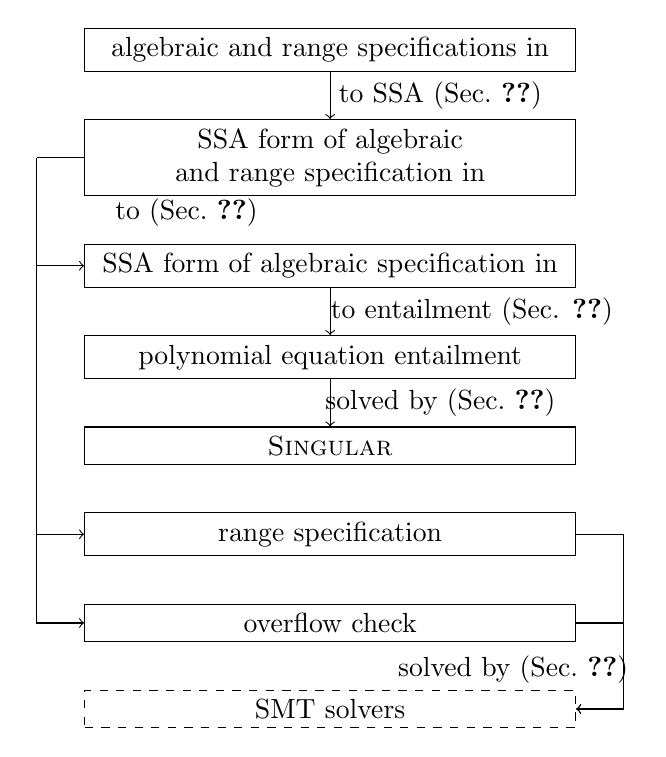
\begin{tikzpicture}[
node distance=0.6cm,
box/.style={rectangle, text width=6cm, fill=white, draw=black},
dot/.style={rectangle, dashed, text width=6cm, fill=white, draw=black},
coord/.style={coordinate},
align=center
]
\node (bvdsl) [box] {algebraic and range specifications in \bvdsl};
\node (bvssa) [box] [below=of bvdsl] {SSA form of algebraic and range specification in \bvdsl};
\node (zssa) [box] [below=of bvssa] {SSA form of algebraic specification in \zdsl};
\node (poly) [box] [below=of zssa] {polynomial equation entailment};
\node (singular) [box] [below=of poly] {\singular};
\node (range) [box] [below=of singular] {range specification};
\node (overflow) [box] [below=of range] {overflow check};
\node (smt) [dot] [below=of overflow] {SMT solvers};
\node (c1) [coord] [left=of bvssa] {};
\node (c2) [coord] [right=of range] {};
\node (c3) [coord] [right=of overflow] {};
\draw[->] (bvdsl) -- node [xshift=1.4cm] {to SSA (Sec.~\ref{subsection:translation:static-single-assignment})} (bvssa);
\draw[-] (bvssa.west) -- node [yshift=-0.7cm,xshift=1.6cm] {to \zdsl (Sec.~\ref{subsection:domain-specific-language-zdsl})} (c1);
\draw[->] (c1) |- node {} (zssa.west);
\draw[->] (c1) |- node {} (range.west);
\draw[->] (c1) |- node {} (overflow.west);
\draw[->] (zssa) -- node  [xshift=1.8cm] {to entailment (Sec. \ref{subsection:translation:multivariant-polynomial-equations})} (poly);
\draw[->] (poly) -- node  [xshift=1.4cm] {solved by (Sec.~\ref{subsection:solving-algebraic-equations})} (singular);
\draw[-] (range.east) -- node {} (c2);
\draw[-] (overflow.east) -- node {} (c3);
\draw[->] (c2) |- node {} (smt.east);
\draw[->] (c3) |- node [xshift=-1.4cm,yshift=0.5cm] {solved by (Sec.~\ref{subsection:solving-range-overflow-checks})} (smt.east);
\end{tikzpicture}
\caption{The verification flow. Except the answers from SMT solvers, all the translations and the answers from \singular are certified by \coq.}
\label{fig:overview}
\end{figure}

We report case studies on verifying mathematical constructs used in
the X25519 ECDH key exchange protocol~\cite{BDL+:11:HSHSS,BDL+:12:HSHSS}.
For each arithmetic operations
(such as addition, subtraction, and multiplication) over $\bbfGF(2^{255} - 19)$,
their low-level real-world implementations are converted to our domain
specific language \bvdsl manually. We specify algebraic properties
of mathematical constructs in Hoare triples. Mathematical constructs
are then verified against their algebraic
specifications with our automatic technique.
The implementation of the Montgomery Ladderstep is
verified similarly.

We have the following contributions:
\begin{itemize}
\item We propose a domain specific language \bvdsl for modeling low-level
  mathematical constructs used in cryptographic programs.
\item We give a certified verification condition generator from
  algebraic specifications of programs to the modular polynomial
  equation entailment problem.
\item We give a certified translation from range problems and overflow checks to SMT formulas.
\item We verify arithmetic computation over a finite field of order
  $2^{255} - 19$ and a
  critical program (the Montgomery Ladderstep) automatically.
\item To the best of our knowledge, our work is the first automatic
  and certified verification on real cryptographic programs with
  minimal human intervention.
\end{itemize}


\noindent
\emph{Related Work}.
Low-level implementations of mathematical constructs have been formalized and manually proved in proof assistants~\cite{Aff13,ANY12,AM07,MG07,M:13:PPVB}.
A semi-automatic approach~\cite{C:14:VCS} has successfully verified a hand-optimized assembly implementation of the Montgomery Ladderstep with SMT solvers, manual program annotation, and a few \coq proofs.
A C implementation of the Montgomery Ladderstep has been automatically verified with \gfverif~\cite{BS:16:GFEV}.
Re-implementations of mathematical constructs in F*~\cite{project:everest} have been verified using a combination of SMT solving and manual proofs.
Several cryptographic implementations in C and Java have been automatically verified by SAW to be equivalent to their reference implementations written in Cryptol~\cite{T:16:AVRWCI} but the correctness of reference implementations is not proven and the verification results are not certified.
The \openssl implementations of SHA-256 and HMAC have been formalized and manually proved in \coq~\cite{A:15:VCPS,B:15:VCSOH}.
Synthesis of assembly codes for mathematical constructs has been proposed in~\cite{fiat:crypto}.
Although the synthesized codes are correct by construction, they are not as efficient as hand-optimized assembly implementations.





\hide{
\cite{AM07} manually prove low-level implementations in SmartMIPS with \coq
\cite{ANY12}
\cite{AFF13} introduce a formalization of data structures for signed multi-precision arithmetic and we experiment it with formal verification of basic functions, using Separation logic
\cite{MG07} Hoare Logic, HOL4, ARM


One approach is to re-implement cryptographic protocols in languages and frameworks that allow efficient verification.
The most extensive work in this area is miTLS, a ``verified reference implementation of the TLS protocol''~\cite{B:14:VRTI,B:13:ITVCS}.
This implementation of TLS is written in F\# and specified in F7 -- the clear focus is on a verifiable (and verified)
re-implementation; not on verifying existing high-speed cryptographic software.
Note that miTLS relies on (unverified)
``cryptographic providers such as .NET or Bouncy Castle''
for core cryptographic primitives.
Also the \cryptver project~\cite{cryptver} aims at re-implementing cryptography such that it can be formally verified.
Their approach is to specify cryptographic algorithms in higher-order logic
and then implement them by formal deductive compilation.

Another approach to formally verified cryptographic software are special-domain compilers.
A recent example of this is~\cite{ABBD13},
where Almeida et al. introduce
\emph{security-aware compilation} of a subset of the C programming language.

The theory of elliptic curve has been formalized in~\cite{TH07,Bar11}.
In principle, the mathematical formulas in Curve25519 Diffie-Hellman
key-exchange can be verified with the formalization.
Low-level machine codes have been formalized in proof
assistants~\cite{Aff13,ANY12,AM07,MG07}. Large-integer arithmetic and
cryptographic functions can be formally verified semi-automatically.
Our approach is very lightweight. Most of the verification is
performed by an SMT solver automatically. It hence requires much less
human intervention.
}

%%% Local Variables:
%%% mode: latex
%%% eval: (TeX-PDF-mode 1)
%%% eval: (TeX-source-correlate-mode 1)
%%% TeX-master: "certified_vcg"
%%% End:



This paper is organized as follows. After preliminaries
(Section~\ref{section:preliminaries}), our domain specific
language is described in Section~\ref{section:domain-specific-language-bvdsl}.
Section~\ref{section:translation}
presents the translation to the algebraic
problem. A certified translation from range and overflow checks to SMT formulas plus a certified solver for the algebraic problem are discussed in Section~\ref{section:verification-of-specifications}.
Section~\ref{section:evaluation} contains experimental results. It is
followed by conclusions.

%%% Local Variables:
%%% mode: latex
%%% eval: (TeX-PDF-mode 1)
%%% eval: (TeX-source-correlate-mode 1)
%%% TeX-master: "certified_vcg"
%%% End:



\section{Preliminaries}
\label{section:preliminaries}

We write $\mathbb{B} = \{ \mathit{ff}, \mathit{tt} \}$ for the Boolean
domain. Let $\bbfN$ and $\bbfZ$ denote all natural numbers and all integers
respectively. We use $[n]$ to denote the set $\{ 0, 1, \ldots, n \}$
for $n \in \bbfN$.

A \emph{monoid} $\mathcal{M} = (M, \epsilon, \cdot)$ consists of a set
$M$ and an associative binary operator $\cdot$ on $M$ with the
\emph{identity} $\epsilon \in M$. That is, $\epsilon \cdot m = m \cdot
\epsilon = m$ for every $m \in M$.
A \emph{group} $\mathcal{G} = (G, 0, +)$ is an algebraic structure
where $(G, 0, +)$ is a monoid and there is a $-a \in G$ such that
$(-a) + a = a + (-a) = 0$ for every $a \in G$. The element $-a$ is
called the \emph{inverse} of $a$. $\mathcal{G}$ is \emph{Abelian} if
the operator $+$ is commutative.
A \emph{ring} $\mathcal{R} = (R, 0, 1, +, \times)$ with $0 \neq 1$ is
an algebraic structure such that
\begin{itemize}
\item $(R, 0, +)$ is an Abelian group; 
\item $(R, 1, \times)$ is a monoid; and 
\item $\times$ is distributive over $+$: $a \times (b + c) = a \times
  b + a \times c$ for every $a, b, c \in R$.
\end{itemize}
If $\times$ is commutative, $\mathcal{R}$ is a \emph{commutative}
ring. 
% An \emph{integral domain} is a commutative ring where $a \times
% b = 0$ implies $a = 0$ or $b = 0$. 
A \emph{field} $\mathcal{F} = (F,
0, 1, +, \times)$ is a commutative ring where $(F\!\setminus\!\{0\}, 1, \times)$ is also
a group. $(\bbfN, 1, \times)$ is a monoid. $(\bbfZ, 0, 1, +, \times)$ 
is a commutative ring but not a field. 
For any prime number $\varrho$, the set $\{ 0, \ldots, \varrho - 1 \}$
with the addition and multiplication modulo $\varrho$ forms a \emph{Galois
field} of order $\varrho$ (written $\bbfGF(\varrho)$).
We focus on Galois fields of very large orders, in particular, $\myprime =
2^{255} - 19$.

Fix a set of variables $\vx$. $\mathcal{R}[\vx]$ is the set of
polynomials over $\vx$ with coefficients in the ring
$\mathcal{R}$. $\mathcal{R}[\vx]$ is a ring. A set $I \subseteq
\mathcal{R}[\vx]$ is an \emph{ideal} if 
\begin{itemize}
\item $f + g \in I$ for every $f, g \in I$; and
\item $h \times f \in I$ for every $h \in
  \mathcal{R}[\vx]$ and $f \in I$. 
\end{itemize}
Given $G \subseteq \mathcal{R}[\vx]$, $\langle G \rangle$ is the
minimal ideal containing $G$; $G$ are the \emph{generators}
of $\langle G \rangle$. The \emph{ideal membership}
problem is to decide if $f \in I$ for a given ideal $I$ and $f
\in \mathcal{R}[\vx]$.

Let $\BV^w$ be the set of all bit-vectors with a bit-width $w$.
The unsigned value of $b \in \BV^w$ is denoted by $\unsigned{b}$.
For a natural number or an integer $n$, let $\bv^w(n)$ be the two's complementation representation of $n$ in a bit-width $w$.
Assume a fixed wordsize $w$ divisible by $4$.
We use $0xn$ to denote a bit-vector $n$ encoded in hexadecimal format.
We use the following common operators for fixed-width bit-vectors: $\BV^w +_\bvop \BV^w : \BV^w$ for addition, $\BV^w -_\bvop \BV^w : \BV^w$ for subtraction, $\BV^w *_\bvop \BV^w : \BV^w$ for multiplication, $\BV^{w_1} ._\bvop \BV^{w_2} : \BV^{w_1 + w_2}$ for concatenation, $\BV^w \#_\bvop n : \BV^{w+n}$ for zero extension, $\BV^w <<_\bvop n : \BV^w$ for left-shifting, $\BV^w >>_\bvop n : \BV^w$ for logical right-shifting, $\hi_\bvop(\BV^{2w}) : \BV^w$ for extraction of high bits, and $\lo_\bvop(\BV^{2w}) : \BV^w$ for extraction of low bits.
Let $b_1$, $b_2$, and $b_3$ be bit-vectors in $\BV^{w}$, and $\bullet \in \{+_\bvop, -_\bvop, *_\bvop\}$.
Define three more operations which perform addition, subtraction, or multiplication after zero extension.
\[
\begin{array}{rcl}
b_1 \bullet^{\#} b_2 & \defn & (b_1 \#_\bvop w) \bullet (b_2 \#_\bvop w) \\
\end{array}
\]
When $\bullet^{\#}$ is applied to more than two bit-vectors, bit-vectors with bit-width already in $2w$ will not be extended again.
For example, $b_1 +_\bvop^{\#} b_2 +_\bvop^{\#} b_3 = (b_1 \#_\bvop w) +_\bvop (b_2 \#_\bvop w) +_\bvop (b_3 \#_\bvop w)$.
Define six more operations which takes high bits or low bits after $\bullet^{\#}$ operation.
\[
\begin{array}{rcl}
b_1 \bullet^{\hi} b_2 & \defn & \hi_\bvop(b_1 \bullet^{\#} b_2) \\
b_1 \bullet^{\lo} b_2 & \defn & \lo_\bvop(b_1 \bullet^{\#} b_2) \\
\end{array}
\]
We also assume comparison operators $<_\bvop$ and $\leq_\bvop$ between unsigned values of bit-vectors.


%%% Local Variables:
%%% mode: latex
%%% eval: (TeX-PDF-mode 1)
%%% eval: (TeX-source-correlate-mode 1)
%%% TeX-master: "certified_vcg"
%%% End:



\section{Domain Specific Language -- \bvdsl}
\label{section:domain-specific-language-bvdsl}

One of the big issues with modern cryptography is how the assumptions
match up with reality. In many situations, unexpected channels
through which information can leak to the attacker may cause the
cryptosystem to be broken. Typically this is about timing or
electric power used.
In side-channel resilient implementations, the execution time
is kept constant (as much as possible) to prevent unexpected
information leakage.
%Implementations which are not defeated through
%such means are called ``side-channel resilient'' implementations.
Constant execution time however is harder to achieve than one would imagine.
%This turns out in some cases to be harder than one would imagine.
%This is chiefly because
Modern processors have caches
%and out of order execution
and multitasking. This makes it possible for one execution
thread, even when no privilege is conferred, to affect the running
time of another -- simply by caching a sufficient amount of its own
data in correct locations through repeated accesses, and then
observing the running time of the other thread. The instructions in
the other thread which use the ``evicted'' data (to make room for the
data of the eavesdropping thread) then have to take more time getting
its data back to the cache~\cite{B:05:CTAA}.
% Such attacks are quite practical.
% \todo{insert reference in bib for D.J. Bernstein ``Cache Timing
% Attacks on AES'', https://cr.yp.to/antiforgery/cachetiming-20050414.pdf}


\hide{
As such, modern cryptographic implementations often have to resort to
seemingly contrived sequences of conditional moves and arithmetic
manipulations to achieve the same result as simply using the CPU
instructions designed for the purpose. This of course slows the
computation down and waste resources but is inevitable because
secret-dependent conditional actions and table lookups are actually
very useful tasks that sometimes simply must be performed.
}

Thus, the innocuous actions of executing (a) a conditional
branch instruction dependent on a secret bit, and (b) an
indirect load instruction using a secret value in the register as the
address, are both potentially dangerous leaks of information.
%There are some side results of the above,
Consequently, we are not often
faced with secret-dependent branching or table-lookups in the assembly
instructions, but a language describing cryptographic code might
include pseudo-instructions to cover instruction sequences, phrases in
the language if you will, that is used to achieve the same effect.
The domain specific language \bvdsl is designed based on the same
principles. Conditional branches and indirect memory accesses are not
admitted in \bvdsl.

Assume some machine architecture with a positive wordsize $\wordsize$.
A program is a straight line of instructions over bit-vectors with bit-width $\wordsize$.
\[
\begin{array}{rcl}
  \Var & ::= & {x} \ |\ {y} \ |\ {z} \ |\ \cdots \\
  \bvAtom & ::= & \Var \ |\ \BV^{\wordsize} \\
  \bvStmt & ::= & \Var \leftarrow \bvAtom \\
          &     & |\ \Var \leftarrow \bvAtom\ {+}\ \bvAtom \\
          &     & |\ \Var\ \Var \leftarrow \bvAtom\ {+}\ \bvAtom \\
          &     & |\ \Var \leftarrow \bvAtom\ {+}\ \bvAtom\ {+}\ \Var \\
          &     & |\ \Var\ \Var \leftarrow \bvAtom\ {+}\ \bvAtom\ {+}\ \Var  \\
          &     & |\ \Var \leftarrow \bvAtom\ {-}\ \bvAtom \\
          &     & |\ \Var \leftarrow \bvAtom\ {\times}\ \bvAtom \\
          &     & |\ \Var\ \Var \leftarrow \bvAtom\ {\times}\ \bvAtom \\
          &     & |\ \Var \leftarrow \bvAtom\ {\ll}\ \BV^{\wordsize} \\
          &     & |\ \Var\ \Var \leftarrow \bvAtom {@} \BV^{\wordsize} \\
          &     & |\ \Var\ \Var \leftarrow (\bvAtom {.} \bvAtom)\ {\ll}\ \BV^{\wordsize}
\end{array}
\]

\begin{figure*}
$
\begin{array}{rcl}
\bvst & \goesto{v \leftarrow a_1 + a_2} & \bvst[v \leftarrow \bvvalueof{a_1}(\bvst) +_\bvop \bvvalueof{a_2}(\bvst)] \\
\bvst & \goesto{c\ v \leftarrow a_1 + a_2} & \bvst[v \leftarrow \lo_\bvop(\bvvalueof{a_1}(\bvst) +_\bvop^\# \bvvalueof{a_2}(\bvst))][c \leftarrow \hi_\bvop(\bvvalueof{a_1}(\bvst) +_\bvop^\# \bvvalueof{a_2}(\bvst))] \\
\bvst & \goesto{v \leftarrow a_1 + a_2 + y} & \bvst[v \leftarrow \lo_\bvop(\bvvalueof{a_1}(\bvst) +_\bvop^\# \bvvalueof{a_2}(\bvst) +_\bvop^\# \bvvalueof{y}(\bvst))] \\
\bvst & \goesto{c\ v \leftarrow a_1 + a_2 + y} & \bvst[v \leftarrow \lo_\bvop(\bvvalueof{a_1}(\bvst) +_\bvop^\# \bvvalueof{a_2}(\bvst) +_\bvop^\# \bvvalueof{y}(\bvst))][c \leftarrow \hi_\bvop(\bvvalueof{a_1}(\bvst) +_\bvop^\# \bvvalueof{a_2}(\bvst) +_\bvop^\# \bvvalueof{y}(\bvst))] \\
\bvst & \goesto{v \leftarrow a_1 - a_2} & \bvst[v \leftarrow \bvvalueof{a_1}(\bvst) -_\bvop \bvvalueof{a_2}(\bvst)] \\
\bvst & \goesto{v \leftarrow a_1 \times a_2} & \bvst[v \leftarrow \bvvalueof{a_1}(\bvst) \times_\bvop \bvvalueof{a_2}(\bvst)] \\
\bvst & \goesto{v_h\ v_l \leftarrow a_1 \times a_2} & \bvst[v_h \leftarrow \hi_\bvop(\bvvalueof{a_1}(\bvst) \times_\bvop^\# \bvvalueof{a_2}(\bvst))][v_l \leftarrow \lo_\bvop(\bvvalueof{a_1}(\bvst) \times_\bvop^\# \bvvalueof{a_2}(\bvst))] \\
\bvst & \goesto{v \leftarrow a \ll n} & \bvst[v \leftarrow \bvvalueof{a}(\bvst) \ll_\bvop \unsigned{n}] \\
\bvst & \goesto{v_h\ v_l \leftarrow a @ n} & \bvst[v_h \leftarrow \bvvalueof{a}(\bvst) \gg_\bvop \unsigned{n}][v_l \leftarrow (\bvvalueof{a}(\bvst) \ll_\bvop (\wordsize -_{\bbfN} \unsigned{n})) \gg_\bvop (\wordsize -_{\bbfN} \unsigned{n})] \\
\bvst & \goesto{v_h\ v_l \leftarrow (a_1 . a_2) \ll n} & \bvst[v_h \leftarrow \hi_\bvop((\bvvalueof{a_1}(\bvst) ._\bvop \bvvalueof{a_2}(\bvst)) \ll_\bvop \unsigned{n})][v_l \leftarrow (\lo_\bvop((\bvvalueof{a_1}(\bvst) ._\bvop \bvvalueof{a_2}(\bvst)) \ll_\bvop \unsigned{n})) \gg_\bvop \unsigned{n}] \\
\end{array}
$
\caption{Transition relation $\bvTr$ for \bvdsl. \label{fig:semantic-function-bvdsl}}
\end{figure*}

Let $\bvSt \defn \Var \rightarrow \BV^{\wordsize}$ and $\bvst \in \bvSt$ be a \emph{state} (or \emph{valuation}).
That is, a {state} $\bvst$ is a mapping from variables to bit-vectors in $\BV^{\wordsize}$.
Define
$
\bvst\mymapsto{v}{d}(u) \defn
\left\{
   \begin{array}{ll}
     d & \textmd{if $u = v$}\\
     \bvst(u) & \textmd{otherwise}
   \end{array}
\right.
$.
Define the semantic function $\bvvalueof{\cdot}(\bvst)$ for variables and atoms as follows.
\[
\begin{array}{rcl}
%\valueof{i}_{\bvst} & \defn & i \textmd{  for ${i} \in \Int$} \\
%\valueof{b}_{\bvst} & \defn & b \textmd{  for ${b} \in \BV^{\wordsize}$} \\
\bvvalueof{v}(\bvst) & \defn & \bvst(v) \textmd{  for ${v} \in \Var$} \\
\bvvalueof{a}(\bvst) & \defn & \left\{
  \begin{array}{ll}
  \bvst(v) & \textmd{if $a$ is a variable $v$} \\
  b & \textmd{if $a$ is a bit-vector $b$} \\
  \end{array}
  \right. \\
\end{array}
\]
Consider the transition relation $\bvTr \subseteq \bvSt \times \bvStmt \times \bvSt$ defined in Figure~\ref{fig:semantic-function-bvdsl} where
$\bvst \goesto{s} \bvst'$ denotes $(\bvst, s, \bvst') \in \bvTr$
for $\bvst, \bvst' \in \bvSt$ and $s \in \bvStmt$.
Basically, $v \leftarrow a_1 + a_2$ is addition, $c\ v \leftarrow a_1 + a_2$ is addition with carry bit placed in $c$, $v \leftarrow a_1 + a_2 + y$ is addition of atoms plus a variable $y$, $c\ v \leftarrow a_1 + a_2 + y$ is addition of atoms plus a variable $y$ with carry bit placed in $c$, $v \leftarrow a_1 - a_2$ is subtraction, $v \leftarrow a_1 \times a_2$ is multiplication, $v_h\ v_l \leftarrow a_1 \times a_2$ is full multiplication, $v \leftarrow a \ll n$ is left-shifting, $v_h\ v_l \leftarrow a @ n$ is splitting at position $n$, and $v_h\ v_l \leftarrow (a_1 . a_2) \ll n$ is left-shifting of higher $n$ bits from $a_2$ to $a_1$.
The variable $y$ in $v \leftarrow a_1 + a_2 + y$ and $c\ v \leftarrow a_1 + a_2 + y$ is intended but not restricted to be carry bits.

A \emph{program} is a sequence of statements.
We denote the empty program by $\epsilon$.
\begin{eqnarray*}
  \bvProg & ::= & \epsilon \ |\ \bvStmt; \bvProg
\end{eqnarray*}
Observe that conditional branches are not allowed in our domain specific language to prevent timing attacks.
The semantics of a program is defined by the relation $\bvTr^* \subseteq \bvSt \times \bvProg \times \bvSt$ where $(\bvst, \epsilon, \bvst) \in \bvTr^*$ and $(\bvst, s; p, \bvst'') \in \bvTr^*$ if there is a $\bvst'$ with $(\bvst, s, \bvst') \in \bvTr$ and $(\bvst', p, \bvst'') \in \bvTr^*$.
We write $\bvst \goesto{p} \bvst'$ when $(\bvst, p, \bvst') \in \bvTr^*$.

For specifications, $\top$ denotes the Boolean value $\mathit{tt}$.
We allow two kinds of specifications, namely algebraic specifications evaluated on domain $\bbfZ$ and range specifications evaluated on domain $\BV^{\wordsize}$.
Atomic predicates in an algebraic specification include polynomial equations $e_1 = e_2$ and modular polynomial equations $e_1 \equiv e_2 \mod e_3$ where $e_i \in \bvExpa$ is a polynomial expression for $i \in \{1, 2, 3\}$.
An \emph{algebraic predicate} $q_a \in \bvPreda$ is then a conjunction of atomic algebraic predicates.
\[
\begin{array}{rcl}
  \bvExpa & ::= & \bbfZ \ |\ \Var \ |\ - \bvExpa \ |\ \bvExpa + \bvExpa \\
          &     & |\ \bvExpa - \bvExpa \ |\ \bvExpa \times \bvExpa \\
  \bvPreda & ::= & \top \ |\ \bvExpa = \bvExpa\ |\ \bvExpa \equiv \bvExpa \mod \bvExpa \\
           &     & |\ \bvPreda \wedge \bvPreda \\
\end{array}
\]
Given a state $\bvst \in \bvSt$ and an expression $e \in \bvExpa$, $\zvalueof{e}(\bvst)$ denotes the value of $e$ on $\bvst$.
\[
\begin{array}{rcl}
  \zvalueof{n}(\bvst) & \defn & n \textmd{ for $n \in \bbfZ$} \\
  \zvalueof{v}(\bvst) & \defn & \unsigned{\bvst(v)} \textmd{ for $v \in \Var$} \\
  \zvalueof{- e}(\bvst) & \defn & -_\bbfZ \zvalueof{e}(\bvst) \\
  \zvalueof{e_1 + e_2}(\bvst) & \defn & \zvalueof{e_1}(\bvst) +_\bbfZ \zvalueof{e_2}(\bvst) \\
  \zvalueof{e_1 - e_2}(\bvst) & \defn & \zvalueof{e_1}(\bvst) -_\bbfZ \zvalueof{e_2}(\bvst) \\
  \zvalueof{e_1 \times e_2}(\bvst) & \defn & \zvalueof{e_1}(\bvst) \times_\bbfZ \zvalueof{e_2}(\bvst) \\
\end{array}
\]
For an algebraic predicate $q_a \in \bvPreda$, we write $\BV^{\wordsize} \models q_a[\bvst]$ if $q_a$ evaluates to $\btt$ using the evaluation function $\zvalueof{e}(\bvst)$ for every subexpression $e$ in $q$.
%For an algebraic predicate $q_a \in \bvPreda$, we write $\BV^{\wordsize} \models q_a[\bvst]$ if one of the following %holds.
%\begin{itemize}
%  \item $q$ is $\top$.
%  \item $q$ is $e_1 = e_2$ and $\zvalueof{e_1}(\bvst)$ equals $\zvalueof{e_2}(\bvst)$.
%  \item $q$ is $e_1 \equiv e_2 \mod e_3$ and $\zvalueof{e_1}(\bvst) \equiv_\bbfZ \zvalueof{e_2}(\bvst) %\mod_\bbfZ \zvalueof{e_3}(\bvst)$.
%  \item $q$ is $q_1 \wedge q_2$, $\BV^{\wordsize} \models q_1$, and $\BV^{\wordsize} \models q_2$.
%\end{itemize}

We admit comparison between atoms in range specifications as atomic range predicates\footnote{In our implementation, comparison between bit-vector expressions is allowed, not only between atoms.}.
A \emph{range predicate} $q_r \in \bvPredr$ is a conjunction of atomic range predicates.
\[
\begin{array}{rcl}
  \bvPredr & ::= & \top \ |\ \bvAtom < \bvAtom \ |\ \bvAtom \leq \bvAtom \\
           &     & |\ \bvPredr \wedge \bvPredr \\
\end{array}
\]
We use $a_l \circ a_1, a_2, \ldots, a_n \bullet a_r$ as a shorthand of the conjunction of $a_l \circ a_1 \wedge a_l \circ a_2 \wedge \cdots \wedge a_l \circ a_n$ and $a_1 \bullet a_r \wedge a_2 \bullet a_r \wedge \cdots \wedge a_n \bullet a_r$ where $\circ, \bullet \in \{<, \leq\}$.
For $q_r \in \bvPredr$ and $\bvst \in \bvSt$, we write $\BV^{\wordsize} \models q_r[\bvst]$ if one of the following holds.
\begin{itemize}
  \item $q$ is $\top$.
  \item $q$ is $a_1 < a_2$ and $\bvvalueof{a_1}(\bvst) <_\bvop \bvvalueof{a_2}(\bvst)$.
  \item $q$ is $a_1 \leq a_2$ and $\bvvalueof{a_1}(\bvst) \leq_\bvop \bvvalueof{a_2}(\bvst)$.
  \item $q$ is $q_1 \wedge q_2$, $\BV^{\wordsize} \models q_1[\bvst]$, and $\BV^{\wordsize} \models q_2[\bvst]$.
\end{itemize}

\begin{figure*}
  \centering
  $
  \begin{array}{lclcl}
    \begin{array}{rcl}
    \textmd{1:} && {r}_0 \leftarrow {x}_0; \\
    \textmd{2:} && {r}_1 \leftarrow {x}_1; \\
    \textmd{3:} && {r}_2 \leftarrow {x}_2; \\
    \textmd{4:} && {r}_3 \leftarrow {x}_3; \\
    \textmd{5:} && {r}_5 \leftarrow {x}_4; \\
    \end{array}
    &\hspace{.05\textwidth}&
    \begin{array}{rcl}
    \textmd{6:} &&
      {r}_0 \leftarrow {r}_0 + {0xFFFFFFFFFFFDA}; \\
    \textmd{7:} &&
      {r}_1 \leftarrow {r}_1 + {0xFFFFFFFFFFFFE}; \\
    \textmd{8:} &&
      {r}_2 \leftarrow {r}_2 + {0xFFFFFFFFFFFFE}; \\
    \textmd{9:} &&
      {r}_3 \leftarrow {r}_3 + {0xFFFFFFFFFFFFE}; \\
    \textmd{10:} &&
      {r}_4 \leftarrow {r}_4 + {0xFFFFFFFFFFFFE}; \\
    \end{array}
    &\hspace{.05\textwidth}&
    \begin{array}{rcl}
    \textmd{11:} && {r}_0 \leftarrow {r}_0 - {y}_0; \\
    \textmd{12:} && {r}_1 \leftarrow {r}_1 - {y}_1; \\
    \textmd{13:} && {r}_2 \leftarrow {r}_2 - {y}_2; \\
    \textmd{14:} && {r}_3 \leftarrow {r}_3 - {y}_3; \\
    \textmd{15:} && {r}_4 \leftarrow {r}_4 - {y}_4;
    \end{array}
  \end{array}
  $
  \caption{Subtraction \dslcode{bSub}}
  \label{figure:dsl:subtraction}
\end{figure*}

A \emph{predicate} $q \in \bvPred$ consists of an algebraic predicate and a range predicate.
\[
\begin{array}{rcl}
  \bvPred & ::= & \bvPreda \andar \bvPredr \\
  \bvSpec & ::= & \cond{\bvPred} \bvProg \cond{\bvPred}
\end{array}
\]
For $\bvst \in \bvSt$ and $q \in \bvPred$, we write $\BV^{\wordsize} \models q[\bvst]$ if $q$ evaluates to $\btt$; $\bvst$ is called a \emph{$q$-state}.
We follow Hoare's formalism in specifications of mathematical constructs~\cite{H:69:ABCP} and call $\hoaretriple{q}{p}{q'}$ a \emph{specification} if $q,q' \in \bvPred$, an \emph{algebraic specification} if $q,q' \in \bvPreda$, and a \emph{range specification} if $q,q' \in \bvPredr$.
In $\hoaretriple{q}{p}{q'}$, $q$ and $q'$ are the \emph{pre}- and \emph{post-conditions} of $p$ respectively.
Given $q, q' \in \bvPred$ ($q,q' \in \bvPreda$, or $q,q' \in \bvPredr$) and $p \in \bvProg$, $\hoaretriple{q}{p}{q'}$ is \emph{valid} (written $\models \hoaretriple{q}{p}{q'}$) if for every $\bvst, \bvst' \in \bvSt$, $\BV^{\wordsize} \models q[\bvst]$ and $\bvst \goesto{p} \bvst'$ imply $\BV^{\wordsize} \models q'[\bvst']$.
Less formally, $\models \hoaretriple{q}{p}{q'}$ if executing $p$ from a $q$-state always results in a $q'$-state.

Given a statement $s \in \bvStmt$ and a state $\bvst \in \bvSt$, the function \textsc{StmtSafe} (Algorithm~\ref{algorithm:stmt-safe}) checks if executing $s$ from $\bvst$ neither overflows nor underflows.
We call a statement $s$ \emph{safe} at a state $\bvst$ if \textsc{StmtSafe}($s$, $\bvst$) evaluates to $\btt$.
A program $p$ is safe at a state $\bvst$, denote by \textsc{ProgSafe}($p$, $\bvst$), if (1) $p = \epsilon$, or (2) $p = s; pp$, \textsc{StmtSafe}($s$, $\bvst$) = $\btt$, and for all $\bvst' \in \bvSt$, $\bvst \goesto{s} \bvst'$ implies \textsc{ProgSafe}($pp$, $\bvst'$).
A program is safe if it is safe at every state.

\begin{algorithm}
  \begin{algorithmic}[1]
    \Function{StmtSafe}{$s$, $\bvst$}
    \Match{$s$}
      \Case{$v \leftarrow a$} \Return $\btt$ \EndCase
      \Case{$v \leftarrow a_1 + a_2$}
        \State{\Return $\hi_\BV(\bvvalueof{a_1}(\bvst) +_\BV^\# \bvvalueof{a_2}(\bvst)) = \bv^\wordsize(0)$}
      \EndCase
      \Case{$c\ v \leftarrow a_1 + a_2$} \Return $\btt$ \EndCase
      \Case{$v \leftarrow a_1 + a_2 + y$}
        \State{\Return $\hi_\BV(\bvvalueof{a_1}(\bvst) +_\BV^\# \bvvalueof{a_2}(\bvst) +_\BV^\# \bvvalueof{y}(\bvst))$}
        \StatexIndent [2] $= \bv^\wordsize(0)$
      \EndCase
      \Case{$c\ v \leftarrow a_1 + a_2 + y$} \Return $\btt$ \EndCase
      \Case{$v \leftarrow a_1 - a_2$}
        \State{\Return $\hi_\BV(\bvvalueof{a_1}(\bvst) -_\BV^\# \bvvalueof{a_2}(\bvst)) = \bv^\wordsize(0)$}
      \EndCase
      \Case{$v \leftarrow a_1 \times a_2$}
        \State{\Return $\hi_\BV(\bvvalueof{a_1}(\bvst) \times_\BV^\# \bvvalueof{a_2}(\bvst)) = \bv^\wordsize(0)$}
      \EndCase
      \Case{$v_h\ v_l \leftarrow a_1 \times a_2$} \Return $\btt$ \EndCase
      \Case{$v \leftarrow a \ll n$}
        \State{\Return $\bvvalueof{a}(\bvst) <_\BV (\bv^\wordsize(1) \ll_\BV (\wordsize -_\bbfN |n|))$}
      \EndCase
      \Case{$v_h\ v_l \leftarrow a @ n$} \Return $\btt$ \EndCase
      \Case{$v_h\ v_l \leftarrow (a_1.a_2) \ll n$}
        \State{\Return $\bvvalueof{a_1}(\bvst) <_\BV (\bv^\wordsize(1) \ll_\BV (\wordsize -_\bbfN |n|)) \wedge$}
        \StatexIndent [2] $|n| \leq_\bbfN \wordsize$
      \EndCase
    \EndMatch
    \EndFunction
  \end{algorithmic}
  \caption{Safety Test for Statements}
  \label{algorithm:stmt-safe}
\end{algorithm}

%\begin{algorithm}
%  \begin{algorithmic}[1]
%    \Function{ProgSafe}{$p$, $\bvst$}
%    \Match{$p$}
%      \Case{$\epsilon$} \Return $\btt$ \EndCase
%      \Case{$s; pp$}
%      \State{\Return \Call{StmtSafe}{$s$, $\bvst$} $\wedge$}
%      \State{\hspace{10mm}$\forall \bvst'. \bvst \goesto{s} \bvst' \implies$\Call{ProgSafe}{$pp$, $\bvst'$}}
%      \EndCase
%    \EndMatch
%    \EndFunction
%  \end{algorithmic}
%  \caption{Safety Test for Programs}
%  \label{algorithm:prog-safe}
%\end{algorithm}

Figure~\ref{figure:dsl:subtraction} gives a simple yet real implementation of subtraction over $\bbfGF(\myprime)$ with a bit-width $64$.
In the figure, a constant bit-vector is written in hexadecimal format starting with the prefix $0x$ and a number in $\bbfGF(\varrho)$ is represented by five bit-vectors each with value less than or equal to $2^{51} +_\bbfZ 2^{15}$.
The variables ${x}_0, {x}_1, {x}_2, {x}_3, {x}_4$ for instance represent $\mathit{radix51}({x}_4, {x}_3, {x}_2, {x}_1, {x}_0) \defn (2^{51 \times 4}) {x}_4 + (2^{51 \times 3}) {x}_3 + (2^{51 \times 2}) {x}_2 + (2^{51 \times 1}) {x}_1 + (2^{51 \times 0}) {x}_0$.
The result of subtraction is stored in the variables ${r}_0, {r}_1, {r}_2, {r}_3, {r}_4$, which are all required to be in the range from $0$ to $2^{54}$.
Let $\mathit{radix51}_\BV({x}_4, {x}_3, {x}_2, {x}_1, {x}_0)$ denote the representation of $\mathit{radix51}({x}_4, {x}_3, {x}_2, {x}_1, {x}_0)$ in $\bvExpa$.
Let $q_a$ $\defn$ $\top$, $q_r$ $\defn$ $0$ $\leq$ ${x}_0,$ ${x}_1,$ ${x}_2,$ ${x}_3,$ ${x}_4,$ ${y}_0,$ ${y}_1,$ ${y}_2,$ ${y}_3,$ ${y}_4$ $\leq$ $\bv^{64}(2^{51} +_\bbfZ 2^{15})$, $q_a'$ $\defn$ $\mathit{radix51}_\BV({x}_4, {x}_3, {x}_2, {x}_1, {x}_0)$ $-$ $\mathit{radix51}_\BV($${y}_4,$ ${y}_3,$ ${y}_2,$ ${y}_1,$ ${y}_0)$ $\equiv$ $\mathit{radix51}_\BV($${r}_4,$ ${r}_3,$ ${r}_2,$ ${r}_1,$ ${r}_0)$ $\mod$ $\myprime$, and $q_r'$ $\defn$ $0$ $\leq$ ${r}_0,$ ${r}_1,$ ${r}_2,$ ${r}_3,$ ${r}_4$ $<$ $\bv^{64}(2^{54})$.
The specification of the mathematical construct is therefore
\[
\begin{array}{rcl}
\cond{q_a \wedge q_r} &
\dslcode{bSub} &
\cond{q_a' \wedge q_r'}.
\end{array}
\]

% 4503599627370458 = 0xFFFFFFFFFFFDA
% 4503599627370494 = 0xFFFFFFFFFFFFE

Note that the variables ${r}_i$'s are added with constants after they are initialized with ${x}_i$'s but before ${y}_i$'s are subtracted from them.
It is not hard to see that
\[
\begin{aligned}
2\myprime = \mathit{radix51} (&\unsigned{0xFFFFFFFFFFFFE}, \unsigned{0xFFFFFFFFFFFFE}, \\
          & \unsigned{0xFFFFFFFFFFFFE}, \unsigned{0xFFFFFFFFFFFFE}, \\
          & \unsigned{0xFFFFFFFFFFFDA})
\end{aligned}
\]
after tedious computation.
Hence
\[
\begin{aligned}
  & \mathit{radix51}({r}_4, {r}_3, {r}_2, {r}_1, {r}_0) \\
= & \mathit{radix51}({x}_4, {x}_3, {x}_2, {x}_1, {x}_0) + 2 \myprime - \mathit{radix51}({y}_4, {y}_3, {y}_2, {y}_1, {y}_0) \\
\equiv & \mathit{radix51}({x}_4, {x}_3, {x}_2, {x}_1, {x}_0) - \mathit{radix51}({y}_4, {y}_3, {y}_2, {y}_1, {y}_0) \mod\ \myprime.
\end{aligned}
\]
The program in Figure~\ref{figure:dsl:subtraction} is correct assuming that it is safe.
Characteristics of large Galois fields are regularly exploited in mathematical constructs for correctness and efficiency.
Our domain specific language can easily model such specialized programming techniques.
Indeed, the reason for adding constants is to prevent underflow.
If the constants were not added, the subtraction in lines~11 to 15 could give negative and hence incorrect results.
We will show how to prove that the program is safe later.

%{Please note that ranges are a complicated
%  issue. The subtraction in Figure~\ref{figure:dsl:subtraction} gives results that are correct
%  but possibly {overflowing} ($>\varrho$), which can and must be
%  accounted for later.}



%\section{Translation to Algebraic Problems}
\section{Transformation of Specifications}
\label{section:translation}

Given $q, q' \in \Pred$ and $p \in \Prog$, we reduce the problem of checking
$\models \hoaretriple{q}{p}{q'}$ to the entailment problem of
polynomial equations over integer variables. The reduction is carried out by
the following three transformations:
\begin{enumerate}
\item Program slicing. To improve efficiency, segments of the program $p$
  irrelevant to the post-condition $q'$ are removed by program slicing 
  (Section~\ref{subsection:translation:slicing}). 
\item Static single assignments. The sliced program is transformed
  into static single assignments. Variables in the pre- and
  post-conditions are renamed accordingly
  (Section~\ref{subsection:translation:static-single-assignment}).
\item Polynomial equations. Validity of algebraic specifications of
  programs in static single assignements is reduced to the entailment
  of a system of polynomial equations
  (Section~\ref{subsection:translation:multivariant-polynomial-equations}). 
\end{enumerate}

For each transformation, we give an algorithm and establish the
correctness of the algorithm in \coq. Specifically, a semantics
for our domain specific language and the validity of algebraic
specifications is formalized in \coq. The correctness of
transformations is then certified by the proof assistant \coq.
For program slicing and static single assignments, we
construct machine-checkable proofs for the soundness and completeness
of the two transformations. For polynomial equations, another
\coq-certified proof shows the soundness of the transformation
from the validity of the algebraic specification to the entailment of 
a system of polynomial equations. In the following subsections,
transformations and their correctness are elaborated in details.  

\subsection{Static Single Assignments}
\label{subsection:translation:static-single-assignment}

A program is in \emph{static single assignment} form if every non-input variable
is assigned at most once and no input variable is assigned~\cite{AWZ:88:DQVP}.
Our next task is to transform any specification
$\hoaretriple{q}{p}{q'}$ to a specification of $p$ in
static single  assignment form for any $q, q' \in \bvPred$ and $p \in
\bvProg$.
To avoid ambiguity, we consider \emph{well-formed} programs where
\begin{itemize}
\item for every statement in the program with two lvalues such as $c\ v \leftarrow a_1 + a_2 + y$ with lvalues $c$ and $v$, the two lvalues are different variables; and
\item every non-input program variable must be assigned to a value
  before being used.
\end{itemize}

Our transformation maintains a finite mapping $\theta$ from variables to
non-negative integers. For any variable $v$, $v^{\theta(v)}$ is
the most recently assigned copy of $v$.
For any atom $a$, $a^{\theta}$ is $v^{\theta(v)}$ when $a$ is a variable $v$, and otherwise is $b$ when $a$ is a constant bit-vector $b$.
Only the most recent copies of variables are referred in
expressions. Algorithm~\ref{algorithm:ssa-expressions}
transforms algebraic expressions with the finite mapping $\theta$ by
structural induction. Integers are unchanged. For each variable, its
most recent copy is returned by looking up the mapping $\theta$. Other
algebraic expressions are transformed recursively.

\begin{algorithm}
  \begin{algorithmic}[1]
    \Function{SSAExpra}{$\theta$, $e$}
    \Match{$e$}
      \Case{$i$} \Return $i$ \EndCase
      \Case{$v$} \Return $v^{\theta(v)}$ \EndCase
      \Case{$-e'$} \Return $-$\Call{SSAExpra}{$\theta$, $e'$} \EndCase
      \Case{$e_1 + e_2$}
        \State{\Return \Call{SSAExpra}{$\theta$, $e_1$} $+$ \Call{SSAExpra}{$\theta$, $e_2$}}
      \EndCase
      \Case{$e_1 - e_2$}
        \State{\Return \Call{SSAExpra}{$\theta$, $e_1$} $-$ \Call{SSAExpra}{$\theta$, $e_2$}}
      \EndCase
      \Case{$e_1 \times e_2$}
        \State{\Return \Call{SSAExpra}{$\theta$, $e_1$} $\times$ \Call{SSAExpra}{$\theta$, $e_2$}}
      \EndCase
    \EndMatch
    \EndFunction
  \end{algorithmic}
  \caption{Static Single Assignment Transformation for Algebraic Expressions}
  \label{algorithm:ssa-expressions}
\end{algorithm}

Similarly, algebraic and range predicates must refer to most recent copies of
variables. They are transformed according to the finite mapping
$\theta$. Thanks to the formalization of finite mappings in \coq. Both
algorithms are easily specified in \gallina.
Let $\textsc{SSAPreda}$ and $\textsc{SSAPredr}$ denote the transformations for $\bvPreda$ and $\bvPredr$ respectively.
The function $\textsc{SSAPred}$ then transforms the algebraic part and the range part of a predicate separatedly with $\textsc{SSAPreda}$ and $\textsc{SSAPredr}$, that is, given $q_a \in \bvPreda$, $q_r \in \bvPredr$, and a mapping $\theta$, $\textsc{SSAPred}(\theta, q_a \andar q_r)$ $\defn$ $\textsc{SSAPreda}(\theta, q_a) \andar \textsc{SSAPredr}(\theta, q_r)$.

\hide{
\begin{algorithm}
  \begin{algorithmic}[1]
    \Function{SSAPreda}{$\theta$, $q$}
    \Match{$q$}
      \Case{$\top$} \Return $\top$ \EndCase
      \Case{$e' = e''$}
        \Return \Call{SSAExpra}{$\theta$, $e$} = \Call{SSAExpra}{$\theta$, $e'$}
      \EndCase
      \Case{$e' \equiv e'' \mod n$}
        \Return \Call{SSAExpra}{$\theta$, $e$} $\equiv$
                \Call{SSAExpra}{$\theta$, $e'$} $\mod n$
      \EndCase
      \Case{$q' \wedge q''$}
        \Return \Call{SSAPreda}{$\theta$, $q'$} $\wedge$
                \Call{SSAPreda}{$\theta$, $q''$}
      \EndCase
    \EndMatch
    \EndFunction
  \end{algorithmic}
  \caption{Static Single Assignment Transformation for Algebraic Predicates}
  \label{algorithm:ssa-predicates}
\end{algorithm}
}

\hide{
\begin{algorithm}
  \begin{algorithmic}[1]
    \Function{SSAAtom}{$\theta$, $a$}
    \Match{$a$}
      \Case{$b$}
        \Return $b$
      \EndCase
      \Case{$v$}
        \Return $v^{\theta(v)}$
      \EndCase
    \EndMatch
    \EndFunction
  \end{algorithmic}
  \caption{Static Single Assignment Transformation for Atoms}
  \label{algorithm:ssa-atoms}
\end{algorithm}
}

\begin{algorithm}
  \begin{algorithmic}[1]
    \Function{SSAStmt}{$\theta$, $s$}
    \Match{$s$}
      \Case{$v \leftarrow a$}
        \State{$\theta' \leftarrow \theta\mymapsto{v}{\theta(v) + 1}$}
        \State{\Return $\langle \theta'$,
                $v^{\theta'(v)} \leftarrow$ $a^\theta$$\rangle$}
      \EndCase
      \Case{$v \leftarrow a_1 + a_2$}
        \State{$\theta' \leftarrow \theta\mymapsto{v}{\theta(v) + 1}$}
        \State{\Return $\langle \theta'$,
                $v^{\theta'(v)} \leftarrow$ $a_1^\theta$ $+$ $a_2^\theta$$\rangle$}
      \EndCase
      \Case{$c\ v \leftarrow a_1 + a_2$}
        \State{$\theta' \leftarrow \theta\mymapsto{c}{\theta(c) + 1}$}
        \State{$\theta'' \leftarrow \theta'\mymapsto{v}{\theta(v) + 1}$}
        \State{\Return $\langle \theta''$,
                $c^{\theta'(c)} \ v^{\theta''(v)} \leftarrow$ $a_1^\theta$ $+$ $a_2^\theta$$\rangle$}
      \EndCase
      \Case{$v \leftarrow a_1 + a_2 + y$}
        \State{$\theta' \leftarrow \theta\mymapsto{v}{\theta(v) + 1}$}
        \State{\Return $\langle \theta'$,
                $v^{\theta'(v)} \leftarrow$ $a_1^\theta$ $+$ $a_2^\theta$ $+$ $y^{\theta(y)}$$\rangle$}
      \EndCase
      \Case{$c\ v \leftarrow a_1 + a_2 + y$}
        \State{$\theta' \leftarrow \theta\mymapsto{c}{\theta(c) + 1}$}
        \State{$\theta'' \leftarrow \theta'\mymapsto{v}{\theta(v) + 1}$}
        \State{\Return $\langle \theta''$,
                $c^{\theta'(c)} \ v^{\theta''(v)} \leftarrow$ $a_1^\theta$ $+$ $a_2^\theta$ $+$ $y^{\theta(y)}$$\rangle$}
      \EndCase
      \Case{$v \leftarrow a_1 - a_2$}
        \State{$\theta' \leftarrow \theta\mymapsto{v}{\theta(v) + 1}$}
        \State{\Return $\langle \theta'$,
                $v^{\theta'(v)} \leftarrow$ $a_1^\theta$ $-$ $a_2^\theta$$\rangle$}
      \EndCase
      \Case{$v \leftarrow a_1 \times a_2$}
        \State{$\theta' \leftarrow \theta\mymapsto{v}{\theta(v) + 1}$}
        \State{\Return $\langle \theta'$,
                $v^{\theta'(v)} \leftarrow$ $a_1^\theta$ $\times$ $a_2^\theta$$\rangle$}
      \EndCase
      \Case{$v_h\ v_l \leftarrow a_1 \times a_2$}
        \State{$\theta' \leftarrow \theta\mymapsto{v_h}{\theta(v_h) + 1}$}
        \State{$\theta'' \leftarrow \theta'\mymapsto{v_l}{\theta(v_l) + 1}$}
        \State{\Return $\langle \theta''$,
                $v_h^{\theta'(v_h)} \ v_l^{\theta''(v_l)} \leftarrow$ $a_1^\theta$ $\times$ $a_2^\theta$$\rangle$}
      \EndCase
      \Case{$v \leftarrow a \ll n$}
        \State{$\theta' \leftarrow \theta\mymapsto{v}{\theta(v) + 1}$}
        \State{\Return $\langle \theta'$,
                $v^{\theta'(v)} \leftarrow$ $a^\theta$ $\ll$ $n$$\rangle$}
      \EndCase
      \Case{$v_h\ v_l \leftarrow a@n$}
        \State{$\theta' \leftarrow \theta\mymapsto{v_h}{\theta(v_h) + 1}$}
        \State{$\theta'' \leftarrow \theta'\mymapsto{v_l}{\theta(v_l) + 1}$}
        \State{\Return $\langle \theta''$,
                $v_h^{\theta'(v_h)} \ v_l^{\theta''(v_l)} \leftarrow$ $a^\theta$ $@$ $n$$\rangle$}
      \EndCase
      \Case{$v_h\ v_l \leftarrow (a_1.a_2) \ll n$}
        \State{$\theta' \leftarrow \theta\mymapsto{v_h}{\theta(v_h) + 1}$}
        \State{$\theta'' \leftarrow \theta'\mymapsto{v_l}{\theta(v_l) + 1}$}
        \State{\Return $\langle \theta''$,
                $v_h^{\theta'(v_h)} \ v_l^{\theta''(v_l)} \leftarrow$ ($a_1^\theta$ $.$ $a_2^\theta$) $@$ $n$$\rangle$}
      \EndCase
    \EndMatch
    \EndFunction
  \end{algorithmic}
  \caption{Static Single Assignment Transformation for Statements}
  \label{algorithm:ssa-statements}
\end{algorithm}

Statement transformation is slightly more complicated
(Algorithm~\ref{algorithm:ssa-statements}). For
atoms and variables on the right hand side, they are transformed by the given
finite mapping $\theta$.
The algorithm of statement transformation then updates $\theta$ and
replaces assigned variables with their latest copies.
%In the algorithm, $\theta\mymapsto{v}{n}$ denotes updating the finite
%mapping $\theta$ by abusing the notation.

\begin{figure*}
  \centering
  $
  \begin{array}{lclcl}
    \begin{array}{rcl}
    \textmd{1:} && {r}^1_0 \leftarrow {x}^0_0; \\
    \textmd{2:} && {r}^1_1 \leftarrow {x}^0_1; \\
    \textmd{3:} && {r}^1_2 \leftarrow {x}^0_2; \\
    \textmd{4:} && {r}^1_3 \leftarrow {x}^0_3; \\
    \textmd{5:} && {r}^1_4 \leftarrow {x}^0_4; \\
    \end{array}
    &\hspace{.05\textwidth}&
    \begin{array}{rcl}
    \textmd{6:} &&
      {r}^2_0 \leftarrow {r}^1_0 + {0xFFFFFFFFFFFDA}; \\
    \textmd{7:} &&
      {r}^2_1 \leftarrow {r}^1_1 + {0xFFFFFFFFFFFFE}; \\
    \textmd{8:} &&
      {r}^2_2 \leftarrow {r}^1_2 + {0xFFFFFFFFFFFFE}; \\
    \textmd{9:} &&
      {r}^2_3 \leftarrow {r}^1_3 + {0xFFFFFFFFFFFFE}; \\
    \textmd{10:} &&
      {r}^2_4 \leftarrow {r}^1_4 + {0xFFFFFFFFFFFFE};\\
    \end{array}
    &\hspace{.05\textwidth}&
    \begin{array}{rcl}
    \textmd{11:} && {r}^3_0 \leftarrow {r}^2_0 - {y}^0_0; \\
    \textmd{12:} && {r}^3_1 \leftarrow {r}^2_1 - {y}^0_1; \\
    \textmd{13:} && {r}^3_2 \leftarrow {r}^2_2 - {y}^0_2; \\
    \textmd{14:} && {r}^3_3 \leftarrow {r}^2_3 - {y}^0_3; \\
    \textmd{15:} && {r}^3_4 \leftarrow {r}^2_4 - {y}^0_4;
    \end{array}
  \end{array}
  $
  \caption{Subtraction \dslcode{bSubSSA} in Static Single Assignment Form}
% $(\dslcode{x}_0, \dslcode{x}_1, \dslcode{x}_2, \dslcode{x}_3,
% \dslcode{x}_4, \dslcode{y}_0, \dslcode{y}_1, \dslcode{y}_2,
% \dslcode{y}_3, \dslcode{y}_4)$
  \label{figure:translation:subtraction-ssa}
\end{figure*}

It is straightforward to transform programs to static single
assignment form (Algorithm~\ref{algorithm:ssa-programs}). Using the
initial mapping $\theta_0$ from variables to $0$,
the algorithm starts from the first statement and obtains an
updated mapping with the statement in static single assignment form. It
continues to transform the next statement with the updated mapping.
Note that our algorithm works for any initial mapping but we choose $\theta_0$ to simplify our \coq proof.

\begin{algorithm}
  \begin{algorithmic}[1]
    \Function{SSAProg}{$\theta$, $p$}
    \Match{$p$}
      \Case{$\epsilon$}
        \Return $\langle \theta,$ $\epsilon \rangle$
      \EndCase
      \Case{$s; pp$}
        \State{$\langle \theta'$, $s' \rangle$ $\leftarrow$
                 \Call{SSAStmt}{$\theta$, $s$}}
        \State{$\langle \theta''$, $pp'' \rangle$ $\leftarrow$
                 \Call{SSAProg}{$\theta'$, $pp$}}
        \State{\Return $\langle \theta''$, $s'; pp'' \rangle$}
      \EndCase
    \EndMatch
    \EndFunction
  \end{algorithmic}
  \caption{Static Single Assignment for Programs}
  \label{algorithm:ssa-programs}
\end{algorithm}

Using the specifications of Algorithm~\ref{algorithm:ssa-statements}
and~\ref{algorithm:ssa-programs} in \gallina, properties of these
algorithms are formally proven in \coq. We first show that
Algorithm~\ref{algorithm:ssa-programs} preserves well-formedness and
produces a program in static single assignment form.
\begin{lemma}
  Let $\theta_0(v) = 0$ for every $v \in \Var$ and $p \in \bvProg$ a well-formed program.
  If $\langle \hat{\theta}, \hat{p} \rangle$ $=
  \textsc{SSAProg}(\theta_0, p)$, then
  $\hat{p}$ is well-formed and in static single assignment form.
  \label{lemma:ssa-programs}
\end{lemma}

The next theorem shows that our transformation is both sound and
complete. That is, a specification is valid if and only if its
corresponding specification in static single assignment form is valid.
\begin{theorem}
  Let $\theta_0(v) = 0$ for every $v \in \Var$.
  For every $q, q' \in \bvPred$ and $p \in \bvProg$,
  \begin{center}
    $\models \hoaretriple{q}{p}{q'}$ if and only if
    $\models \hoaretriple{\textsc{SSAPred}(\theta_0, q)}
    {\hat{p}}
    {\textsc{SSAPred}(\hat{\theta}, q')}$
  \end{center}
  where $\langle \hat{\theta}, \hat{p} \rangle =
  \textsc{SSAProg}(\theta_0, p)$.
  \label{theorem:ssa}
\end{theorem}

\noindent
\emph{Example.}
Figure~\ref{figure:translation:subtraction-ssa} gives the subtraction program
\dslcode{bSub} in static single assignment form. Starting from $0$, the
index of a variable is incremented when the variable is assigned to an
expression. After the static single assignment translation, the
variables ${x}_i$'s, ${y}_i$'s are indexed by $0$ and
${r}_i$'s are indexed by $3$ for $0 \leq i \leq 4$.
Subsequently, variables in pre- and post-conditions of the
specification for subtraction need to be indexed.
Let $\hat{q}_a$ $\defn$ $\top$, $\hat{q}_r$ $\defn$ $0$ $\leq$ ${x}^0_0,$ ${x}^0_1,$ ${x}^0_2,$ ${x}^0_3,$ ${x}^0_4,$ ${y}^0_0,$ ${y}^0_1,$ ${y}^0_2,$ ${y}^0_3,$ ${y}^0_4$ $\leq$ $\bv^{64}(2^{51} +_\bbfZ 2^{15})$, $\hat{q}_a'$ $\defn$ $\mathit{radix51}_\BV({x}^0_4, {x}^0_3, {x}^0_2, {x}^0_1, {x}^0_0)$ $-$ $\mathit{radix51}_\BV({y}^0_4, {y}^0_3, {y}^0_2, {y}^0_1, {y}^0_0)$ $\equiv$ $\mathit{radix51}_\BV({r}^3_4, {r}^3_3, {r}^3_2, {r}^3_1, {r}^3_0)$ $\mod$ $\myprime$, and $q_r'$ $\defn$ $0$ $\leq$ ${r}^3_0,$ ${r}^3_1,$ ${r}^3_2,$ ${r}^3_3,$ ${r}^3_4$ $<$ $\bv^{64}(2^{54})$.
The corresponding specification of in static single assignment form is then
\[
\cond{\hat{q}_a \wedge \hat{q}_r} \dslcode{bSubSSA} \cond{\hat{q}_a' \wedge \hat{q}_r'}.
\]

\hide{
\[
\begin{array}{rcl}
\cond{\hat{q}_a \wedge \hat{q}_r} &
\dslcode{bSubSSA} &
\cond{\hat{q}_a' \wedge \hat{q}_r'}.
\end{array}
\]
}


\subsection{\zdsl}
\label{subsection:domain-specific-language-zdsl}

One of the big issues with modern cryptography is how the assumptions
match up with reality. In many situations, unexpected channels
through which information can leak to the attacker can cause the
cryptosystem to be broken. Typically this is about timing, or
electric power used. Implementations which are not defeated through
such means are called ``side-channel resilient'' implementations.
Clearly in such implementations the execution time are kept constant
(as much as possible).

This turns out in some cases to be harder than one would imagine.
This is chiefly because modern processors have caches and out of order
execution and multitasking. This makes it possible for one execution
thread, even when no privilege is conferred ,to affect the running
time of another -- simply by caching a sufficient amount of its own
data in correct locations through repeated accesses, and then
observing the running time of the other thread. The instructions in
the other thread which uses the ``evicted'' data (to make room for the
data of the eavesdropping thread) then has to take more time getting
their data back to the cache. Such attacks are quite practical.
\todo{insert reference to cache-timing attacks.}

Thus, the innocuous actions of (a) executing the CPU's conditional
branch instruction dependent on a secret bit, and (b) executing an
indirect load instruction using a secret value in the register as the
address, are both potentially dangerous leaks of information.

As such, modern cryptographic implementations often have to resort to
seemingly contrived sequences of conditional moves and arithmetic
manipulations to achieve the same result as simply using the CPU
instructions designed for the purpose. This of course slows the
computation down and waste resources but is inevitable because
secret-dependent conditional actions and table lookups are actually
very useful tasks that sometimes simply must be performed.

There are some side results of the above, one is that we are not often
faced with secret-dependent branching or table-lookups in the assembly
instructions, but a language describing cryptographic code might
include pseudo-instructions to cover instruction sequences, phrases in
the language if you will, that is used to achieve the same effect.

Consider the following syntactic class for expressions in our domain
specific language:

\begin{eqnarray*}
  N & ::= & \dslcode{1}\ |\ \dslcode{2}\ |\ \cdots\\
  Z & ::= & \cdots \ |\ \dslcode{-2}\ |\ \dslcode{-1} \ |\ 0\ |\ 
            \dslcode{1}\ |\ \dslcode{2}\ |\ \cdots\\
  V & ::= & \dslcode{x} \ |\ \dslcode{y} \ |\ \dslcode{z} \ |\ \cdots\\
  E & ::= &  Z \ |\ V \ |\  \dslcode{-}E \ |\ E \dslcode{+} E 
             \ |\ E \dslcode{-} E
             \ |\ E \times E \ |\ \dslcode{Pow} (E, N)
\end{eqnarray*}

We allow exact integers as constants in the domain specific
language. Variables are thus integer variables. An expression can be a
constant, a variable, or a negative expression. Addition, subtraction,
and multiplication of expressions are available. The expression
$\dslcode{Pow}(e, n)$ denotes $e^n$ for any expression $e$ and positive
integer $n$. More formally, let $\St \defn V \rightarrow
\bbfZ$ and $\nu \in \St$ be a \emph{state}. That is,
a {state} $\nu$ is a mapping from variables to integers. Define the
semantic function $\valueof{e}_{\nu}$ for an expression $e$ as follows.
\[
\begin{array}{rclcrcl}
  \valueof{{i}}_{\nu} & \defn & i \textmd{  for ${i} \in Z$} 
  & \hspace{.1\textwidth} &
  \valueof{{v}}_{\nu} & \defn & \nu({v}) 
     \textmd{  for ${v} \in V$}\\
  \valueof{-e}_{\nu} & \defn & -_{\bbfZ}\valueof{e}_{\nu}
  &&
  \valueof{e_0 + e_1}_{\nu} & \defn & 
     \valueof{e_0}_{\nu} +_{\bbfZ} \valueof{e_1}_{\nu} \\
  \valueof{e_0 - e_1}_{\nu} & \defn & 
     \valueof{e_0}_{\nu} -_{\bbfZ} \valueof{e_1}_{\nu}
  &&
  \valueof{e_0 \times e_1}_{\nu} & \defn & 
     \valueof{e_0}_{\nu} \times_{\bbfZ} \valueof{e_1}_{\nu} \\
  \valueof{\dslcode{Pow}(e, n)}_{\nu} & \defn & 
     (\valueof{e}_{\nu})^{\valueof{n}_{\nu}}
\end{array}
\]

Note that there is no expression for quotients, bitwise logical
operations. Bitwise left shifting however can be modeled by
multiplying $\dslcode{Pow}(2, n)$. Although \mydsl models a (very) 
small subset of assembly, it suffices to encode crucial low-level
mathematical constructs in X25519.

\begin{eqnarray*}
  S & ::= & V \leftarrow E 
            \ |\  \concat{V}{V} \leftarrow \dslcode{Split} (E, N)\\
\end{eqnarray*}

For low-level mathematical constructs, only assignments are allowed.
The statement $v \leftarrow e$ assigns the value of $e$
to the variable $v$. The statement $\concat{v_h}{v_l} \leftarrow
\dslcode{Split}(e, n)$ splits the value of $e$ into two parts;
the lowest $n$ bits are stored in $v_l$ and the higher bits
are stored in $v_h$. Define
\begin{eqnarray*}
\nu[\vv \mapsto \vd](v) & \defn &
\left\{
   \begin{array}{ll}
     d_i & \textmd{if $v = v_i \in \vv$}\\
     \nu(v) & \textmd{otherwise}
   \end{array}
\right.
\end{eqnarray*}
Consider the relation $\Tr \subseteq \St \times S \times \St$ defined
as follows. 
\begin{eqnarray*}
  (\nu, v \leftarrow e, \nu') \in \Tr & \textmd{if} &
  \nu' = \nu[v \mapsto \valueof{e}_{\nu}]\\
  (\nu, \concat{v_h}{v_l} \leftarrow \dslcode{Split} (e, n), \nu') \in
  \Tr & \textmd{if} &
  \nu' = \nu[v_h, v_l \mapsto h, l]
\end{eqnarray*}
where
$l = \valueof{e}_{\nu} \mod 2^{\valueof{n}_{\nu}}$ and
$h = (\valueof{e}_{\nu} - l) \div 2^{\valueof{n}_{\nu}}$.
Hence $(\nu, s, \nu') \in \Tr$ denotes that the state $\nu$ transits to 
the state $\nu'$ after executing the statement $s$.

\begin{eqnarray*}
  P & ::= & \epsilon \ |\ S; P
\end{eqnarray*}

A program is a sequence of statements. We denote the empty program by
$\epsilon$. Observe that conditional branches are not allowed in
cryptographic programs to prevent timing attacks. The semantics of a
program is defined by the relation 
$\Tr^* \subseteq \St \times P \times \St$:
\begin{eqnarray*}
  (\nu, \epsilon, \nu) \in \Tr^*\\
  (\nu, s; p, \nu'') \in \Tr^* & \textmd{if} &
    \textmd{there is a } \nu' \textmd{ with }
    (\nu, s, \nu') \in \Tr^* \textmd{ and }
    (\nu, p, \nu'') \in \Tr^*.
\end{eqnarray*}
Let $\nu, \nu' \in \St$ and $p = s_1; s_2; \cdots; s_n \in
P$. $\nu'$ is a state after executing $p$ from $\nu$
(written $\nu \goesto{p} \nu'$) if there are $\nu_1 = \nu, \nu_2,
\ldots, \nu_n, \nu_{n+1} = \nu'$ with $(\nu_i, s_i, \nu_{i+1}) \in
\Tr^*$ for every $1 \leq i < n$.

For algebraic specifications, $\top$ denotes the Boolean value
$\mathit{tt}$. A \emph{predicate} $q \in Q$ is an arbitrary
conjunction of (modulo) equations over expressions are admissible. For
$\nu \in \St$, we write $\bbfZ \models q[\nu]$ if $q$
evaluates to $\btt$ after replacing each variable $v$ with
$\nu(v)$; $\nu$ is moreover called a \emph{$q$-state}.

\begin{eqnarray*}
  Q & ::= & \top
     \ |\   E = E
     \ |\   E \equiv E \mod N
     \ |\   Q \wedge Q\\
  H & ::= & \cond{Q} P \cond{Q}
\end{eqnarray*}

We follow Hoare's formalism in algebraic specifications of
mathematical constructs~\cite{H:69:ABCP}. In an algebraic
specification $\hoaretriple{q}{p}{q'}$, $q$ and $q'$ are the \emph{pre}- and
\emph{post-conditions} of $p$ respectively. Given $q, q' \in Q$ and $p
\in P$, $\models \hoaretriple{q}{p}{q'}$ if for every $\nu, \nu' \in
\St$, $\bbfZ \models q[\nu]$ and $\nu \goesto{p} \nu'$ imply
$\bbfZ \models q'[\nu']$. Less formally, $\models
\hoaretriple{q}{p}{q'}$ if executing $p$ from a $q$-state always
results in a $q'$-state.

\begin{figure}[ht]
  \centering
  \[
  \begin{array}{lclcl}
    \begin{array}{rcl}
    \textmd{1:} && \dslcode{r}_0 \leftarrow \dslcode{x}_0; \\
    \textmd{2:} && \dslcode{r}_1 \leftarrow \dslcode{x}_1; \\
    \textmd{3:} && \dslcode{r}_2 \leftarrow \dslcode{x}_2; \\
    \textmd{4:} && \dslcode{r}_3 \leftarrow \dslcode{x}_3; \\
    \textmd{5:} && \dslcode{r}_5 \leftarrow \dslcode{x}_4; \\
    \end{array}
    &\hspace{.05\textwidth}&
    \begin{array}{rcl}
    \textmd{6:} && 
      \dslcode{r}_0 \leftarrow \dslcode{r}_0 + \dslcode{4503599627370458}; \\
    \textmd{7:} &&
      \dslcode{r}_1 \leftarrow \dslcode{r}_1 + \dslcode{4503599627370494}; \\
    \textmd{8:} &&
      \dslcode{r}_2 \leftarrow \dslcode{r}_2 + \dslcode{4503599627370494}; \\
    \textmd{9:} &&
      \dslcode{r}_3 \leftarrow \dslcode{r}_3 + \dslcode{4503599627370494}; \\
    \textmd{10:} && 
      \dslcode{r}_4 \leftarrow \dslcode{r}_4 + \dslcode{4503599627370494};\\
    \end{array}
    &\hspace{.05\textwidth}&
    \begin{array}{rcl}
    \textmd{11:} && \dslcode{r}_0 \leftarrow \dslcode{r}_0 - \dslcode{y}_0; \\
    \textmd{12:} && \dslcode{r}_1 \leftarrow \dslcode{r}_1 - \dslcode{y}_1; \\
    \textmd{13:} && \dslcode{r}_2 \leftarrow \dslcode{r}_2 - \dslcode{y}_2; \\
    \textmd{14:} && \dslcode{r}_3 \leftarrow \dslcode{r}_3 - \dslcode{y}_3; \\
    \textmd{15:} && \dslcode{r}_4 \leftarrow \dslcode{r}_4 - \dslcode{y}_4;
    \end{array}
  \end{array}
  \]
  \caption{Subtraction \dslcode{sub}}
%$(\dslcode{x}_0, \dslcode{x}_1, \dslcode{x}_2, \dslcode{x}_3,
%\dslcode{x}_4, \dslcode{y}_0, \dslcode{y}_1, \dslcode{y}_2,
%\dslcode{y}_3, \dslcode{y}_4)$
  \label{figure:dsl:subtraction}
\end{figure}

Figure~\ref{figure:dsl:subtraction} gives a simple yet real
implementation of subtraction over $\bbfGF(\myprime)$. 
In the figure, a number in $\bbfGF(\varrho)$ 
is represented by five 51-bit unsigned integers. The variables
$\dslcode{x}_0, \dslcode{x}_1, \dslcode{x}_2, \dslcode{x}_3,
\dslcode{x}_4$ for instance represent 
$\mathit{radix51}(\dslcode{x}_4, \dslcode{x}_3, \dslcode{x}_2,
\dslcode{x}_1, \dslcode{x}_0) \defn
2^{51 \times 4} \dslcode{x}_4 + 2^{51 \times 3} \dslcode{x}_3 + 
2^{51 \times 2} \dslcode{x}_2 + 2^{51 \times 1} \dslcode{x}_1 + 
2^{51 \times 0} \dslcode{x}_0$. The result of
subtraction is stored in the variables $\dslcode{r}_0, \dslcode{r}_1,
\dslcode{r}_2, \dslcode{r}_3, \dslcode{r}_4$. 
Given $0 \leq \dslcode{x}_0,$ $\dslcode{x}_1,$ $\dslcode{x}_2,$
$\dslcode{x}_3,$ $\dslcode{x}_4,$ $\dslcode{y}_0,$ $\dslcode{y}_1,$
$\dslcode{y}_2,$ $\dslcode{y}_3,$ $\dslcode{y}_4 < 2^{51}$, 
the specification of the program is therefore
\[
\begin{array}{c}
\cond{\top}\\
\dslcode{sub}\\
%(\dslcode{x}_0, \dslcode{x}_1, \dslcode{x}_2, \dslcode{x}_3,
%\dslcode{x}_4, \dslcode{y}_0, \dslcode{y}_1, \dslcode{y}_2,
%\dslcode{y}_3, \dslcode{y}_4)\\
\cond{\mathit{radix}(\dslcode{x}_4, \dslcode{x}_3, \dslcode{x}_2,
\dslcode{x}_1, \dslcode{x}_0) -
\mathit{radix51}(\dslcode{y}_4, \dslcode{y}_3, \dslcode{y}_2,
\dslcode{y}_1, \dslcode{y}_0)
\equiv
\mathit{radix51}(\dslcode{r}_4, \dslcode{r}_3, \dslcode{r}_2,
\dslcode{r}_1, \dslcode{r}_0)
\mod \myprime
}.
\end{array}
\]

Note that the variables $\dslcode{r}_i$'s are added with constants
after they are initizlied with $\dslcode{x}_i$'s but before
$\dslcode{y}_i$'s are subtracted from them. It is not hard to see that
$2\myprime = \mathit{radix51} (4503599627370458,$ $4503599627370494,$
$4503599627370494,$ $4503599627370494,$ $4503599627370494)$
after tedious computation. Hence $\mathit{radix51}(\dslcode{r}_4,$
$\dslcode{r}_3,$ $\dslcode{r}_2,$ $\dslcode{r}_1,$ $\dslcode{r}_0)$ $=$
$\mathit{radix51}(\dslcode{x}_4,$ $\dslcode{x}_3,$ $\dslcode{x}_2,$
$\dslcode{x}_1,$ $\dslcode{x}_0)$ $+$ $2 \myprime $ $-$
$\mathit{radix51}(\dslcode{y}_4,$ $\dslcode{y}_3,$ $\dslcode{y}_2,$
$\dslcode{y}_1,$ $\dslcode{y}_0)$ $\equiv $
$\mathit{radix51}(\dslcode{x}_4,$ $\dslcode{x}_3,$ $\dslcode{x}_2,$
$\dslcode{x}_1,$ $\dslcode{x}_0)$ $-$
$\mathit{radix51}(\dslcode{y}_4,$ $\dslcode{y}_3,$ $\dslcode{y}_2,$
$\dslcode{y}_1,$ $\dslcode{y}_0)$ $\mod \myprime $. The program in
Figure~\ref{figure:dsl:subtraction} is correct. The reason for
adding constants is to prevent underflow. If the constants were not
added, the subtraction in lines~11 to 15 could give negative and hence
incorrect results. Indeed, characteristics of large Galois fields are
regularly exploited in cryptographic programs for correctness and
efficiency. Our domain specific language can easily model such
specialized programming techniques and is most suitable for low-level
cryptographic programs.


%\subsection{Program Slicing}
%\label{subsection:translation:slicing}
%
Consider the problem of checking whether $\hoaretriple{q}{p}{q'}$ for
arbitrary $q, q' \in Q$ and $p \in P$. Since $q'$ is arbitrary, the
program $p$ may contain fragments irrevelant to $q'$. Program slicing
is a simple yet effective technique to improve efficiency of
verification through simplifying programs. \todo{reference?} 

Here we slice programs in a backward manner. We initialize the set
of \emph{cared} variables to be the variables appeared in the
post-condition $q'$. Starting from the last statement, we check if
it assigns any cared variables. If not, we skip the last statement and
move to the last but one statement. If it does, we keep the last
statement, update the cared variables, and examine the second-to-last
statement. This process repeats until the first statement of the
program is processed.

Our program slicing algorithm requires several auxiliary functions. 
Algorithm~\ref{algorithm:variables-in-expressions} shows how to
compute all variables occurred in an expression by a structural
induction on the expression. If the given expression is an integer,
the empty set is returned; if it is a variable, the singleton with the
variable is returned. Variables in other expressions are computed
recursively. 

\begin{algorithm}
  \begin{algorithmic}[1]
    \Function{VarsInExpr}{$e$}
    \Match{$e$}
      \Case{$v$}
        \Return $\{ v \}$
      \EndCase
      \Case{$i$}
        \Return $\emptyset$
      \EndCase
      \Case{$-e'$}
        \Return \Call{VarsInExpr}{$e'$}
      \EndCase
      \Case{$e' + e''$}
        \Return \Call{VarsInExpr}{$e'$} $\cup$ \Call{VarsInExpr}{$e''$}
      \EndCase
      \Case{$e' - e''$}
        \Return \Call{VarsInExpr}{$e'$} $\cup$ \Call{VarsInExpr}{$e''$}
      \EndCase
      \Case{$e' \times e''$}
        \Return \Call{VarsInExpr}{$e'$} $\cup$ \Call{VarsInExpr}{$e''$}
      \EndCase
      \Case{$\dslcode{Pow}(e', \uscore)$}
        \Return \Call{VarsInExpr}{$e'$}
      \EndCase
    \EndMatch
    \EndFunction
  \end{algorithmic}
  \caption{Variables Occurred in Expressions}
  \label{algorithm:variables-in-expressions}
\end{algorithm}

\begin{algorithm}
\begin{algorithmic}[1]
  \Function{VarsInPred}{$q$}
  \Match{$q$}
    \Case{$\top$}
      $\emptyset$
    \EndCase
    \Case{$e' = e''$}
      \Return \Call{VarsInExpr}{$e'$} $\cup$ \Call{VarsInExpr}{$e''$}
    \EndCase
    \Case{$e' \equiv e'' \mod \uscore$}
      \Return \Call{VarsInExpr}{$e'$} $\cup$ \Call{VarsInExpr}{$e''$}
    \EndCase
    \Case{$q' \wedge q''$}
      \Return \Call{VarsInPred}{$q'$} $\cup$ \Call{VarsInPred}{$q''$}
    \EndCase
  \EndMatch
  \EndFunction
\end{algorithmic}
\caption{Variables Occurred in Predicates}
\label{algorithm:variables-in-predicates}
\end{algorithm}

Similarly, Algorithm~\ref{algorithm:variables-in-predicates} computes
the variables appeared in a predicate. Using the \coq specification
langauge \gallina, both algorithms are specified in the proof
assistant easily. 

\begin{algorithm}
  \begin{algorithmic}[1]
    \Function{SliceStatement}{$\mathit{vars}$, $s$}
    \Match{$s$}
      \Case{$v \leftarrow e$}
        \IfThenElse{$v \in \mathit{vars}$}
          {\Return $\langle$\Call{VarsInExpr}{$e$} 
            $\cup$ $(\mathit{vars} \setminus \{ v \})$, $s \rangle$}
          {\Return $\mathit{vars}$}
      \EndCase
      \Case{$\concat{v_h}{v_l} \leftarrow \dslcode{Split} (e, \uscore)$}
        \IfThenElse{$v_h$ or $v_l \in \mathit{vars}$}
          {\Return $\langle$\Call{VarsInExpr}{$e$} $\cup$ 
            $(\mathit{vars} \setminus \{ v_h, v_l \})$, $s \rangle$}
          {\Return $\mathit{vars}$}
      \EndCase
    \EndMatch
    \EndFunction
  \end{algorithmic}
  \caption{Slicing Statements}
  \label{algorithm:slicing-statements}
\end{algorithm}

For each statement, we check if the variables in the left hand side are
cared variables. If these variables are not, we leave the cared
variables intact. If they are cared variables, we update the cared
variables by excluding the variables on the left hand side but adding
the variables appeared on the right hand
side~(Algorithm~\ref{algorithm:slicing-statements}). In the algorithm, 
the parameter $\mathit{vars}$ denotes the set of cared variables.
Observe that irrelevant statements are not returned by the algorithm.

To slice a program, our algorithm proceeds from the last statement
(Algorithm~\ref{algorithm:slicing-programs}). It invokes
\textsc{SliceStatement} to see if the current statement is relevant
and update cared variables if necessary. The algorithm recurses with
the updated cared variables and all but the last statements.

\begin{algorithm}
  \begin{algorithmic}[1]
    \Function{SliceProgram}{$\mathit{vars}$, $p$}
    \Match{$p$}
      \Case{$\epsilon$}
        \Return $\epsilon$
      \EndCase
      \Case{$pp; s;$}
        \Match{\Call{SliceStatement}{$\mathit{vars}$, $s$}}
          \Case{$\mathit{vars}'$}
            \Return \Call{SliceProgram}{$\mathit{vars}'$, $pp;$}
          \EndCase
          \Case{$\langle \mathit{vars}'$, $s' \rangle$}
            \Return \Call{SliceProgram}{$\mathit{vars}'$, $pp$}$\ s';$
          \EndCase
        \EndMatch
      \EndCase
    \EndMatch
    \EndFunction
  \end{algorithmic}
  \caption{Slicing Programs}
  \label{algorithm:slicing-programs}
\end{algorithm}

We specify Algorithms~\ref{algorithm:slicing-statements}
and~\ref{algorithm:slicing-programs} in \gallina. Their properties are
also specified and proven formally in \coq. Particularly, the
soundness and completeness of our program slicing algorithm have been
established in the proof assistant. That is, the proof of the
following theorem is certified. 

\begin{theorem}
  For every $q, q' \in Q$ and $p \in P$,
  \begin{center}
  $\models \hoaretriple{q}{p}{q'}$ if and only if
  $\models \hoaretriple{q}{\textsc{SliceProgram}(\textsc{VarsInPred}(q'), p)}
  {q'}$.
  \end{center}
  \label{theorem:program-slicing}
\end{theorem}

\subsection{Modular Polynomial Equation Entailment}
\label{subsection:translation:multivariant-polynomial-equations}

The last step transforms any algebraic program specification in \zdsl to the
modular polynomial equation entailment problem. For
$q \in \zPred$, we write $q(\vx)$ to signify the free variables $\vx$
occurred in $q$. Given $q(\vx), q'(\vx) \in \zPred$, the \emph{modular
  polynomial equation entailment} problem decides whether
$q(\vx) \implies q'(\vx)$ holds when $\vx$ are substituted for
arbitrary integers. That is, we want to check if for every valuation $\zst \in \zSt$, $q(\vx)$ evaluates to $\btt$ implies $q'(\vx)$ evaluates to $\btt$ after each variable $x$ is replaced by $\zst(x)$.
We write $\bbfZ \models \forall \vx. q(\vx) \implies q'(\vx)$ if it is indeed the case.

Programs in static single assignment form can easily be transformed to
conjunctions of polynomial equations. An assignment statement is
translated to a polynomial equation with a variable on the left hand side.
A $\dslcode{Split}$ statement is transformed to an
equation with a linear expression of the assigned variables on the
left hand side (Algorithm~\ref{algorithm:polynomial-statements}).
\begin{algorithm}
  \begin{algorithmic}[1]
    \Function{StmtToPolyEQ}{$s$}
    \Match{$s$}
      \Case{$v \leftarrow e$}
        \Return $v = e$
      \EndCase
      \Case{$\concat{v_h}{v_l} \leftarrow \dslcode{Split}(e, n)$}
        \State{\Return $v_l + \dslcode{Pow}(2, n) \times v_h = e$}
      \EndCase
    \EndMatch
    \EndFunction
  \end{algorithmic}
  \caption{Polynomial Equation Transformation for Statements}
  \label{algorithm:polynomial-statements}
\end{algorithm}

A program in static single assignment form is transformed to the
conjunction of polynomial equations corresponding to its statements
(Algorithm~\ref{algorithm:polynomial-programs}).

\begin{algorithm}
  \begin{algorithmic}[1]
    \Function{ProgToPolyEQ}{$p$}
    \Match{$p$}
      \Case{$\epsilon$} \Return $\top$ \EndCase
      \Case{$s; pp$}
        \State{\Return \Call{StmtToPolyEQ}{$s$} $\wedge$ \Call{ProgToPolyEQ}{$pp$}}
      \EndCase
    \EndMatch
    \EndFunction
  \end{algorithmic}
  \caption{Polynomial Equation Transformation for Programs}
  \label{algorithm:polynomial-programs}
\end{algorithm}

Algorithm~\ref{algorithm:polynomial-statements}
and~\ref{algorithm:polynomial-programs} are specified straightforwardly
in \gallina. We use the proof assistant \coq to prove properties
about the algorithms. Note that $\textsc{ProgToPolyEQ}(p) \in
\zPred$ for every $p \in \zProg$. The following theorem shows that any
behavior of the program $p$ is a solution to the system of polynomial
equations $\textsc{ProgToPolyEQ}(p)$. In other words,
$\textsc{ProgToPolyEQ}(p)$ gives an abstraction of the program $p$.

\begin{theorem}
  Let $p \in \zProg$ be a well-formed program in static single assignment
  form. For every $\zst, \zst' \in \zSt$ with $\zst \goesto{p} \zst'$,
  we have $\bbfZ \models \textsc{ProgToPolyEQ}(p) [\zst']$.
\end{theorem}

Definition~\ref{definition:program-entailment} gives the modular
polynomial equation entailment problem corresponding to an algebraic
program specification.
\begin{definition}
  For $q, q' \in \zPred$ and $p \in \zProg$ in static single assignment
  form, define
  \begin{eqnarray*}
    \Pi(\hoaretriple{q}{p}{q'}) & \defn &
    q(\vx) \wedge \varphi(\vx) \implies q'(\vx)
  \end{eqnarray*}
  where $\varphi(\vx) =
  \textsc{ProgToPolyEQ}(p)$.
  \label{definition:program-entailment}
\end{definition}

\begin{figure*}
  \centering
  $
  \begin{array}{l}
  \top \wedge
  \left(
  \begin{array}{lclcl}
    \begin{array}{rclc}
      {r}^1_0 & = & {x}^0_0 & \wedge \\
      {r}^1_1 & = & {x}^0_1 & \wedge \\
      {r}^1_2 & = & {x}^0_2 & \wedge \\
      {r}^1_3 & = & {x}^0_3 & \wedge \\
      {r}^1_4 & = & {x}^0_4 & \wedge \\
    \end{array}
    &\hspace{.01\textwidth}&
    \begin{array}{rclc}
      {r}^2_0 & = & {r}^1_0 + {4503599627370458} & \wedge \\
      {r}^2_1 & = & {r}^1_1 + {4503599627370494} & \wedge \\
      {r}^2_2 & = & {r}^1_2 + {4503599627370494} & \wedge \\
      {r}^2_3 & = & {r}^1_3 + {4503599627370494} & \wedge \\
      {r}^2_4 & = & {r}^1_4 + {4503599627370494} & \wedge\\
    \end{array}
    &\hspace{.01\textwidth}&
    \begin{array}{rclc}
      {r}^3_0 & = & {r}^2_0 - {y}^0_0 & \wedge \\
      {r}^3_1 & = & {r}^2_1 - {y}^0_1 & \wedge \\
      {r}^3_2 & = & {r}^2_2 - {y}^0_2 & \wedge \\
      {r}^3_3 & = & {r}^2_3 - {y}^0_3 & \wedge \\
      {r}^3_4 & = & {r}^2_4 - {y}^0_4
    \end{array}
  \end{array}
  \right) \implies \\
    %\hspace{.05\textwidth}
    \mathit{radix51}_\bbfZ({x}^0_4, {x}^0_3, {x}^0_2, {x}^0_1, {x}^0_0) -
    \mathit{radix51}_\bbfZ({y}^0_4, {y}^0_3, {y}^0_2, {y}^0_1, {y}^0_0)
    \equiv
    \mathit{radix51}_\bbfZ({r}^3_4, {r}^3_3, {r}^3_2, {r}^3_1, {r}^3_0)
    \mod \myprime
  \end{array}
  $
  \caption{Modular Polynomial Equation Entailment for \textsc{BV2ZProg}(\dslcode{bSubSSA})}
  \label{figure:translation:subtraction-polynomial}
\end{figure*}

\noindent
\emph{Example}.
The modular polynomial equation entailment problem corresponding to the
algebraic specification of subtraction is shown in
Figure~\ref{figure:translation:subtraction-polynomial}. The problem
has 15 polynomial equality constraints with 25 variables.
Define $\mathit{radix51}_\bbfZ({x}_4, {x}_3, {x}_2, {x}_1, {x}_0) \defn \dslcode{Pow}(2, 51 \times_\bbfZ 4) \times {x}_4 + \dslcode{Pow}(2, 51 \times_\bbfZ 3) \times {x}_3 + \dslcode{Pow}(2, 51 \times_\bbfZ 2) \times {x}_2 + \dslcode{Pow}(2, 51 \times_\bbfZ 1) \times {x}_1 + \dslcode{Pow}(2, 51 \times_\bbfZ 0) \times {x}_0$ for ${x}_0, {x}_1, {x}_2, {x}_3, {x}_4 \in \Var$.
We want to know if $\mathit{radix51}_\bbfZ({r}^3_4, {r}^3_3, {r}^3_2,
{r}^3_1, {r}^3_0)$ is the difference between $\mathit{radix51}_\bbfZ({x}^0_4,
{x}^0_3, {x}^0_2, {x}^0_1, {x}^0_0)$ and $\mathit{radix51}_\bbfZ({y}^0_4,
{y}^0_3, {y}^0_2, {y}^0_1, {y}^0_0)$ in $\bbfGF(\varrho)$ under the
constraints.

The soundness of Algorithm~\ref{algorithm:polynomial-programs}
is certified in \coq (Theorem~\ref{theorem:program-to-q-soundness}).
% Its proof is again certified by \coq.
\begin{theorem}
  \label{theorem:program-to-q-soundness}
  Let $q, q' \in \zPred$ be predicates, and $p \in \zProg$ a well-formed
  program in static single assignment form.
  If $\bbfZ \models \forall \vx.\Pi(\hoaretriple{q}{p}{q'})$, then
  $\models$ $\hoaretriple{q}{p}{q'}$.
\end{theorem}


\subsubsection*{Summary of Translation}

Consider any predicates $q_a, q_a' \in \bvPreda$, $q_r, q_r' \in \bvPredr$, and well-formed program $p \in
\bvProg$. Let $\theta_0 (v) = 0$ for every $v \in \Var$. By
Theorem~\ref{theorem:ssa}, \ref{theorem:bv2z}, and \ref{theorem:program-to-q-soundness}, we have a summary of translation in Figure~\ref{fig:summary}.
Observe that $\tilde{p}$ in Figure~\ref{fig:summary} is well-formed and in static single assignment
form (Lemma~\ref{lemma:ssa-programs} and \ref{lemma:bv2z-prog}).
Theorem~\ref{theorem:program-to-q-soundness} is applicable in the last
deduction. After the translations, a safety check, a range problem, and an instance of the modular
polynomial equation entailment problem are obtained from the given
specification of a well-formed program in \bvdsl.
To verify mathematical constructs against their specifications, we will solve all the three problems in the next section.

\begin{figure}
\[
  \begin{array}{cll}
    & \models \hoaretriple{q_a \andar q_r}{p}{q_a' \andar q_r'}\\
%    \Leftrightarrow
%    & \models
%      \hoaretriple{q}{\textsc{SliceProg}(\textsc{VarsInPred}(q'), p)}{q'}
%    & \textmd{ (Theorem~\ref{theorem:program-slicing})}\\
    \Leftrightarrow
    & \models
      \hoaretriple{\hat{q}_a \andar \hat{q}_r}
      {\hat{p}}
      {\hat{q}_a' \andar \hat{q}_r'}
    & \textmd{ (Theorem~\ref{theorem:ssa})}\\
    &
      \textmd{where } \langle \hat{\theta}, \hat{p} \rangle =
      \textsc{SSAProg} (\theta_0, p), \\
    & \hat{q}_a = \textsc{SSAPreda}(\theta_0, q_a), \\
    & \hat{q}_r = \textsc{SSAPredr}(\theta_0, a_r), \\
    & \hat{q}_a' = \textsc{SSAPreda}(\hat{\theta}, q_a'), \textmd{ and} \\
    & \hat{q}_r' = \textsc{SSAPredr}(\hat{\theta}, q_r') \\
    \Leftarrow
    & \multicolumn{2}{l}{\BV^\wordsize \models \hat{q}_r[\bvst] \textmd{ implies } \textsc{ProgSafe}(\hat{p}) = \btt \textmd{ for all } \bvst \in \bvSt,} \\
    & \models \hoaretriple{\hat{q}_r}{\hat{p}}{\hat{q}_r'}, \textmd{ and } \\
    & \models \hoaretriple{\tilde{q}_a}{\tilde{p}}{\tilde{q}_a'}
    & \textmd{ (Theorem~\ref{theorem:bv2z})} \\
    & \textmd{where } \tilde{p} = \textsc{BV2ZProg}(\hat{p}), \\
    & \tilde{q}_a = \textsc{BV2ZPred}(\hat{q}_a), \textmd{ and} \\
    & \tilde{q}_a' = \textsc{BV2ZPred}(\hat{q}_a') \\
    \Leftarrow
    & \multicolumn{2}{l}{\BV^\wordsize \models \hat{q}_r[\bvst] \textmd{ implies } \textsc{ProgSafe}(\hat{p}) = \btt \textmd{ for all } \bvst \in \bvSt,} \\
    & \models \hoaretriple{\hat{q}_r}{\hat{p}}{\hat{q}_r'}, \textmd{ and } \\
    & \bbfZ \models \forall \vx.
      \Pi (\hoaretriple{\tilde{q}_a}{\tilde{p}}{\tilde{q}_a'})
    & \textmd{ (Theorem~\ref{theorem:program-to-q-soundness})}
  \end{array}
\]
  \caption{Summary of Translations}
  \label{fig:summary}
\end{figure}

\hide{
\begin{equation*}
  \begin{array}{cll}
    & \models \hoaretriple{q_a \wedge q_r}{p}{q_a' \wedge q_r'}\\
%    \Leftrightarrow
%    & \models
%      \hoaretriple{q}{\textsc{SliceProg}(\textsc{VarsInPred}(q'), p)}{q'}
%    & \textmd{ (Theorem~\ref{theorem:program-slicing})}\\
    \Leftrightarrow
    & \models
      \hoaretriple{\hat{q}_a \wedge \hat{q}_r}
      {\hat{p}}
      {\hat{q}_a' \wedge \hat{q}_r'}
    & \textmd{ (Theorem~\ref{theorem:ssa})}\\
    &
      \textmd{where } \langle \hat{\theta}, \hat{p} \rangle =
      \textsc{SSAProg} (\theta_0, p), \\
    & \hat{q}_a = \textsc{SSAPred}(\theta_0, q_a), \\
    & \hat{q}_r = \textsc{SSAPred}(\theta_0, a_r), \\
    & \hat{q}_a' = \textsc{SSAPred}(\hat{\theta}, q_a'), \textmd{ and} \\
    & \hat{q}_r' = \textsc{SSAPred}(\hat{\theta}, q_r') \\
    \Leftarrow
    & \multicolumn{2}{l}{\BV^\wordsize \models \hat{q}_r[\bvst] \textmd{ implies } \textsc{ProgSafe}(\hat{p}) = \btt \textmd{ for all } \bvst \in \bvSt,} \\
    & \models \hoaretriple{\hat{q}_r}{\hat{p}}{\hat{q}_r'}, \textmd{ and } \\
    & \models \hoaretriple{\tilde{q}_a}{\tilde{p}}{\tilde{q}_a'}
    & \textmd{ (Theorem~\ref{theorem:bv2z})} \\
    & \textmd{where } \tilde{p} = \textsc{BV2ZProg}(\hat{p}), \\
    & \tilde{q}_a = \textsc{BV2ZPred}(\hat{q}_a), \textmd{ and} \\
    & \tilde{q}_a' = \textsc{BV2ZPred}(\hat{q}_a') \\
    \Leftarrow
    & \multicolumn{2}{l}{\BV^\wordsize \models \hat{q}_r[\bvst] \textmd{ implies } \textsc{ProgSafe}(\hat{p}) = \btt \textmd{ for all } \bvst \in \bvSt,} \\
    & \models \hoaretriple{\hat{q}_r}{\hat{p}}{\hat{q}_r'}, \textmd{ and } \\
    & \bbfZ \models \forall \vx.
      \Pi (\hoaretriple{\tilde{q}_a}{\tilde{p}}{\tilde{q}_a'})
    & \textmd{ (Theorem~\ref{theorem:program-to-q-soundness})}
  \end{array}
\end{equation*}
}



\section{Verification of Specifications}
\label{section:verification-of-specifications}

We show how to solve a range problem, check if a program is safe, and solve modular polynomial equation
entailment problem in this section.
The first two problems are reduced to QF\_BV formulas and solved by an SMT solver.
The last problem is reduced to an ideal membership problem and solve by the computer algebra system \singular.

\subsection{Solving Range and Overflow Checks}
\label{subsection:solving-range-overflow-checks}

First define the syntax of a fragment of QF\_BV.
In this fragment, a variable always represents a bit-vector of bit-width $\wordsize$ (the assumed wordsize).
Let $\qExp$ and $\qPred$ respectively denote the expressions and the predicates in QF\_BV.
An expression $e \in \qExp$ can be a constant $\bvconst(n, b)$, a variiable $v \in \Var$, an addition $\bvadd(e_1, e_2)$, a subtraction $\bvsub(e_1, e_2)$, a multiplication $\bvmul(e_1, e_2)$, a concatenation $\bvconcat(e_1, e_2)$, a zero extension $\bvext(e', i)$, a left-shifting $\bvshl(e_1, e_2)$, a logical right-shifting $\bvlshr(e_1, e_2)$, or an extraction $\bvextract(e', i, j)$ where $n, i, j \in \bbfN$, $b \in \BV^n$, and $e_1, e_2, e' \in \qExp$.
A predicate $q \in \qPred$ can be an equality $e_1 = e_2$, a less-than $\bvult(e_1, e_2)$, a less-then-or-equal $\bvule(e_1, e_2)$, a negation $\neg q'$, a conjunction $q_1 \wedge q_2$, or a disjunction $q_1 \vee q_2$ where $e_1, e_2 \in \qExp$ and $q', q_1, q_2 \in \qPred$.
An implication $q_1 \Rightarrow q_2$ is defined as $\neg q_1 \vee q_2$.

Let $\max(n, m)$ return the maximal number in $n$ and $m$.
Given an expression $e \in \qExp$, $\width(e)$ denotes the maximal bit-width of $e$.
\[
\begin{array}{rcl}
\width(\bvconst(n, b)) & = & n \\
\width(v) & = & w \\
\width(\bvadd(e_1, e_2)) & = & max(\width(e_1), \width(e_2))\\
\width(\bvsub(e_1, e_2)) & = & max(\width(e_1), \width(e_2))\\
\width(\bvmul(e_1, e_2)) & = & max(\width(e_1), \width(e_2))\\
\width(\bvconcat(e_1, e_2)) & = & \width(e_1) +_\bbfN \width(e_2)\\
\width(\bvext(e, i)) & = & \width(e) +_\bbfN i \\
\width(\bvshl(e_1, e_2)) & = & \width(e_1) \\
\width(\bvlshr(e_1, e_2)) & = & \width(e_1) \\
\width(\bvextract(e, i, j)) & = & i -_\bbfN j +_\bbfN 1 \\
\end{array}
\]
The expression $e$ is called \emph{well-formed} if $e$ is (1) a constant, a variable, a concatenation, a zero extension, a left-shifting, or a logical right-shifting, (2) an addition $\bvadd(e_1, e_2)$, a subtraction $\bvsub(e_1, e_2)$, or a multiplication $\bvmul(e_1, e_2)$ with $\width(e_1) = \width(e_2)$ and both $e_1$ and $e_2$ well-formed, or (3) an extraction $\bvextract(e', i, j)$ with $0 \leq j \leq i < \width(e')$ and $e'$ well-formed.
A predicate $q \in \qPred$ is well-formed if all sub-expressions are well-formed.

Let $\bvst \in \bvSt$ be a state.
Define the semantic function $\bvvalueof{e}(\bvst)$ for well-formed expressions $e$.
\[
\begin{array}{rcl}
\bvvalueof{\bvconst(n, b)}(\bvst) & \defn & b \\
\bvvalueof{v}(\bvst) & \defn & \zvalueof{v}(\bvst) \\
\bvvalueof{\bvadd(e_1, e_2)}(\bvst) & \defn & \bvvalueof{e_1}(\bvst) +_\BV \bvvalueof{e_2}(\bvst) \\
\bvvalueof{\bvsub(e_1, e_2)}(\bvst) & \defn & \bvvalueof{e_1}(\bvst) -_\BV \bvvalueof{e_2}(\bvst) \\
\bvvalueof{\bvmul(e_1, e_2)}(\bvst) & \defn & \bvvalueof{e_1}(\bvst) \times_\BV \bvvalueof{e_2}(\bvst) \\
\bvvalueof{\bvconcat(e_1, e_2)}(\bvst) & \defn & \bvvalueof{e_1}(\bvst) ._\BV \bvvalueof{e_2}(\bvst) \\
\bvvalueof{\bvext(e, i)}(\bvst) & \defn & \bvvalueof{e}(\bvst) \#_\BV i \\
\bvvalueof{\bvshl(e_1, e_2)}(\bvst) & \defn & \bvvalueof{e_1}(\bvst) \ll_\BV |\bvvalueof{e_2}(\bvst)| \\
\bvvalueof{\bvlshr(e_1, e_2)}(\bvst) & \defn & \bvvalueof{e_1}(\bvst) \gg_\BV |\bvvalueof{e_2}(\bvst)| \\
\bvvalueof{\bvextract(e, i, j)}(\bvst) & \defn & \bvvalueof{e}(\bvst)[i, j] \\
\end{array}
\]
For a predicate $q \in \qPred$, we write $\BV^{\wordsize} \models q[\bvst]$ if $q$ evaluates to $\btt$ using the evaluation function $\bvvalueof{e}(\bvst)$ for every subexpression $e$ in $q$, using $<_\BV$ for $\bvult$, and using $\leq_\BV$ for $\bvule$.

Now we are ready to convert overflow/underflow checks and range problems to QF\_BV.
Let $q_r, q_r' \in \bvPredr$ be two range predicates and $p \in \bvProg$ a well-formed program in static single assignment form.
Both an overflow/underflow check ($\BV^\wordsize \models q_r[\bvst]$ implies $\textsc{ProgSafe}(p, \bvst) = \btt$ for all $\bvst \in \bvSt$) and a range problem ($\models \hoaretriple{q_r}{p}{q_r'}$) involve only bit-vector operations and can be easily modeled by QF\_BV expressions according to the semantics of $\textsc{ProgSafe}$, programs, range predicates, and range specifications.
To save space, we only show some examples.
Define $\textsc{AtomToQFBV}(a)$ as $v$ if the atom $a$ is a variable $v$ and otherwise $\bvconst(w, b)$ if $a$ is a constant $b$.
Let $\textsc{ProgToQFBV}(p)$ be the representing formula of $p$ in QF\_BV such that $\bvst \goesto{p} \bvst'$ implies $\BV^\wordsize \models \textsc{ProgToQFBV}(p)[\bvst']$.
For example, $\textsc{ProgToQFBV}($ $v$ $\leftarrow$ $a_1$ $+$ $a_2)$ is $v$ $=$ $\textsc{AtomToQFBV}(a_1)$ $+_\BV$ $\textsc{AtomToQFBV}(a_2)$ and $\textsc{ProgToQFBV}($$v_h\ v_l \leftarrow a @ n)$ is $v_h$ $=$ $\textsc{AtomToQFBV}(a)$ $\gg_\BV$ $\bv^w(n)$ $\wedge$ $v_l$ $=$ $(\textsc{AtomToQFBV}(a)$ $\ll_\BV$ $\bv^w(w - n))$ $\gg_\BV$ $\bv^w(w - n)$.
Let $\textsc{SafeToQFBV}(p)$ be the representing formula for $\textsc{ProgSafe}$ such that $\textsc{ProgSafe}(p, \bvst) = \btt$ if and only if $\BV^\wordsize \models \textsc{SafeToQFBV}(p)$.
Let $\textsc{PredrToQFBV}(q_r)$ be the representing formula for a $q_r \in \bvPredr$ such that $\BV^\wordsize \models q_r$ if and only if $\BV^\wordsize \models \textsc{PredrToQFBV}(q_r)$.
The following theorem states the soundness of our translation from range problems and overflow/underflow checks to QF\_BV.

\begin{theorem}
Given two range predicates $q_r, q_r' \in \bvPredr$ and a well-formed program $p \in \bvProg$ in static single assignment form,
\begin{itemize}
\item $\BV^\wordsize \models q_r[\bvst]$ implies $\textsc{ProgSafe}(p, \bvst) = \btt$ for all $\bvst \in \bvSt$ if, $(\textsc{PredrToQFBV}(q_r) \wedge \textsc{ProgToQFBV}(p)) \Rightarrow \textsc{SafeToQFBV}(p)$ is valid, and
\item $\models \hoaretriple{q_r}{p}{q_r'}$ if $\textsc{PredrToQFBV}(q_r) \wedge \textsc{ProgToQFBV}(p) \Rightarrow \textsc{PredrToQFBV}(q_r')$ is valid.
\end{itemize}
\label{theorem:to-qfbv}
\end{theorem}







\subsection{Solving Modular Polynomial Equation Entailment Problem}
\label{subsection:solving-algebraic-equations}

By Theorem~\ref{theorem:program-to-q-soundness}, it remains to show 
that 
\[
\begin{array}{l}
  \forall \vx. % \in \bbfZ^{|\vx|}.
  \bigwedge\limits_{i \in [I]} e_i (\vx) = e'_i (\vx) \wedge
  \bigwedge\limits_{j \in [J]} f_j (\vx) \equiv f'_j (\vx) \mod n_j
  \implies
  \\
  \hspace{.3\textwidth}
  \bigwedge\limits_{k \in [K]} g_k (\vx) = g'_k (\vx) \wedge
  \bigwedge\limits_{l \in [L]} h_l (\vx) \equiv h'_l (\vx) \mod m_l
\end{array}
\]
where
$e_i (\vx), e'_i (\vx), f_j (\vx), f'_j (\vx),
 g_k (\vx), g'_k (\vx), h_l (\vx), h'_l (\vx) \in
 \bbfZ[\vx]$, $n_j, m_l \in \bbfN$ for $i \in [I]$, $j \in [J]$, $k
 \in [K]$, and $l \in [L]$. Since the
implicant is a conjunction of (modulo) equations, it suffces to 
prove one conjunct at a time. That is, we aim to show that 
\begin{equation}
  \label{eq:polynomial-equation-implicant}
  \forall \vx. % \in \bbfZ^{|\vx|}.
  \bigwedge\limits_{i \in [I]} e_i (\vx) = e'_i (\vx) \wedge
  \bigwedge\limits_{j \in [J]} f_j (\vx) \equiv f'_j (\vx) \mod n_j
  \implies
  g (\vx) = g' (\vx)
\end{equation}
where $e_i (\vx), e'_i (\vx), f_j (\vx), f'_j (\vx), g (\vx), g' (\vx)
\in \bbfZ[\vx]$ for $i \in [I], j \in [J]$; or, 
 \begin{equation}
   \label{eq:modular-polynomial-equation-implicant}
   \forall \vx. % \in \bbfZ^{|\vx|}.
   \bigwedge\limits_{i \in [I]} e_i (\vx) = e'_i (\vx) \wedge
   \bigwedge\limits_{j \in [J]} f_j (\vx) \equiv f'_j (\vx) \mod n_j
   \implies
   h (\vx) \equiv h' (\vx) \mod m
 \end{equation}
where $e_i (\vx), e'_i (\vx), f_j (\vx), f'_j (\vx), h (\vx), h' (\vx)
\in \bbfZ[\vx]$ for $i \in [I], j \in [J]$, and $m \in \bbfN$. 

It is not hard to rewrite modular polynomial equations in antecedents
in (\ref{eq:polynomial-equation-implicant}) and 
(\ref{eq:modular-polynomial-equation-implicant}) to polynomial
equations~\cite{H:07:AENTP}. By definition of modular polynomial equations,
(\ref{eq:polynomial-equation-implicant}) is equivalent to
\[
\forall \vx. % \in \bbfZ^{|\vx|}.
\bigwedge\limits_{i \in [I]} e_i (\vx) = e'_i (\vx) \wedge
\bigwedge\limits_{j \in [J]} [\exists d_j. f_j (\vx) = f'_j (\vx) + d_j \cdot n_j]
\implies
g (\vx) = g' (\vx),
\]
which in turn is equivalent to
\[
\forall \vx \vd. % \in \bbfZ^{|\vx|} \vd \in \bbfZ^{J}.
\bigwedge\limits_{i \in [I]} e_i (\vx) = e'_i (\vx) \wedge
\bigwedge\limits_{j \in [J]} f_j (\vx) = f'_j (\vx) + d_j \cdot n_j
\implies
g (\vx) = g' (\vx).
\]

\hide{
Consider the following system of $r + s$ (modulo) equations:
\begin{equation}
  \label{equation:modulo-polynomials}
  \begin{array}{rclcrcl}
    e_1 (\vx) & = & e'_1 (\vx) 
    & \hspace{.05\textwidth} &
    f_1 (\vx) & \equiv & f'_1 (\vx) \mod n_1\\
    & \vdots & & & & \vdots \\
    e_i (\vx) & = & e'_i (\vx) & &
    f_j (\vx) & \equiv & f'_j (\vx) \mod n_j\\
    & \vdots & & & & \vdots \\
    e_r (\vx) & = & e'_r (\vx) & &
    f_s (\vx) & \equiv & f'_s (\vx) \mod n_s
  \end{array}
\end{equation}
Our goal is to establish $g (\vx) = g' (\vx)$ or $h (\vx)
\equiv h (\vx) \mod m$ for every $\vx$ satisfying the system
of equations~(\ref{equation:modulo-polynomials}). In order to prove it
in \coq, we first rewrite modulo equations $f_j (\vx) \equiv f'_j
(\vx) \mod n_j$ to existentially quantified equations $\exists d_j
\in \bbfZ, f_j (\vx) = f'_j (\vx) + n_j \times d_j$. In other
words, we want to show that for every $\vx \in \bbfZ^{|\vx|}$
satisfying 
\begin{equation}
  \label{equation:polynomials}
  \begin{array}{rclcrcl}
    e_1 (\vx) & = & e'_1 (\vx) 
    & \hspace{.05\textwidth} &
    f_1 (\vx) & = & f'_1 (\vx) + n_1 \times d_1 \\
    & \vdots & & & & \vdots \\
    e_i (\vx) & = & e'_i (\vx) & &
    f_j (\vx) & = & f'_j (\vx) + n_j \times d_j \\
    & \vdots & & & & \vdots \\
    e_r (\vx) & = & e'_r (\vx) & &
    f_s (\vx) & = & f'_s (\vx) + n_s \times d_s
  \end{array}
\end{equation}
with some $d_1, \ldots, d_s$, then $g (\vx) = g' (\vx)$ or $h
(\vx) \equiv h' (\vx) \mod m$. 
}

In other words, it suffices to consider the following
\emph{polynomial equation entailment} problems~\cite{H:07:AENTP}:
\begin{equation}
  \label{eq:reduced-polynomial-equation-implicant}
  \forall \vx. % \in \bbfZ^{|\vx|}.
  \bigwedge\limits_{i \in [I]} e_i (\vx) = e'_i (\vx)
  \implies
  g (\vx) = g' (\vx)
\end{equation}
where $e_i (\vx), e'_i (\vx), g (\vx), g' (\vx) \in \bbfZ[\vx]$ for $i
\in [I]$; or,
 \begin{equation}
   \label{eq:reduced-modular-polynomial-equation-implicant}
   \forall \vx. % \in \bbfZ^{|\vx|}.
   \bigwedge\limits_{i \in [I]} e_i (\vx) = e'_i (\vx)
   \implies
   h (\vx) \equiv h' (\vx) \mod m
 \end{equation}
where $e_i (\vx), e'_i (\vx), h (\vx), h' (\vx) \in \bbfZ[\vx]$ for $i
\in [I]$ and $m \in \bbfN$.

One way to solve the polynomial equation entailment problems
~(\ref{eq:reduced-polynomial-equation-implicant})
and~(\ref{eq:reduced-modular-polynomial-equation-implicant}) is by
solving the ideal membership problem~\cite{H:07:AENTP,BS:16:GFEV}. 
For~(\ref{eq:reduced-polynomial-equation-implicant}), consider the
ideal $I = \langle e_i(\vx) - e'_i(\vx) \rangle_{i \in [I]}$. Suppose
$g(\vx) - g'(\vx) \in I$. Then there are $u_i(\vx) \in \bbfZ[\vx]$
such that 
\[
g(\vx) - g'(\vx) = \sum\limits_{i \in [I]} u_i (\vx) [e_i (\vx) - e' (\vx)].
\]
Hence $g(\vx) - g'(\vx) = 0$ by the polynomial equations $e_i (\vx) =
e' (\vx)$ for $i \in [I]$ in the antecedents
in~(\ref{eq:reduced-polynomial-equation-implicant}). Similarly, it
suffices to check if $h(\vx) - h'(\vx) \in \langle m, e_i(\vx) -
e'_i(\vx) \rangle_{i \in [I]}$
for~(\ref{eq:reduced-modular-polynomial-equation-implicant}).
The reduction to the ideal membership problem however is sound but
incomplete. There are instances
of~(\ref{eq:reduced-polynomial-equation-implicant})
or~(\ref{eq:reduced-modular-polynomial-equation-implicant}) whose
corresponding ideal membership problems do not hold. 

The ideal membership problem can be solved by finding a Gr\"obner
basis for the ideal. There are two \coq tactics to
construct formal proofs for the polynomial equation entailment
problems~(\ref{eq:reduced-polynomial-equation-implicant})
and~(\ref{eq:reduced-modular-polynomial-equation-implicant})~\cite{P:08:CGBP,P:10:CGBP}. 
The tactic \dslcode{nsatz} is able to prove
equalities in integral domains. The tactic \dslcode{gbarith} is able
to prove modulo equalities in integral domains. We define a
\coq tactic which invokes \dslcode{nsatz} or \dslcode{gbarith} 
to prove $g (\vx) = g' (\vx)$ or $h (\vx) \equiv
h' (\vx) \mod m$ respectively. Finding Gr\"obner bases for ideals is
%
NP-complete, because finding Gr\"obner basis allows us to
  solve a system of equations, which is NP-complete even for the
  boolean field~\cite{GJ:1979:CAI}.
%
The tactics \dslcode{nsatz} and \dslcode{gbarith} are not very
scalable.
For modulo arithmetic over large finite fields, their 
implementations can have hundreds of polynomial equations
in~(\ref{eq:reduced-polynomial-equation-implicant})
or~(\ref{eq:reduced-modular-polynomial-equation-implicant}). 
The \coq tactics are unable to finish
the proof in a reasonable amount of time. A more scalable tactic is
necessary to verify implementations of low-level cryptographic codes.

For the polynomial equations generated by \textit{ProgramToQ}
($p$) (Algorithm~\ref{algorithm:polynomial-programs}), they are of the
following forms: $x = E$ (from an assignment statement) or $x + 2^c y
= E$ (from a \dslcode{Split} statement). Such polynomial equations can
safely be removed after every occurrences of $x$ are replaced with $E$
or $E - 2^c y$. The number of polynomial equations is thus greatly
reduced. We hence define a \coq tactic to rewrite variables and then
remove corresponding polynomial equations. For proving a polynomial
equation $g (\vx) = g' (\vx)$, it turns out that the \coq tactic
\dslcode{ring} suffices. For a modulo equation $h (\vx) \equiv
h' (\vx) \mod m$, \todo{we need what?}

%%% Local Variables: 
%%% mode: latex
%%% eval: (TeX-PDF-mode 1)
%%% eval: (TeX-source-correlate-mode 1)
%%% TeX-master: "certified_vcg"
%%% End: 



\section{Evaluation}
\label{section:evaluation}

We evaluate our techniques in real-world low-level cryptographic
programs. In elliptic curve cryptography, arithmetic computation over
large finite fields is required for cryptographic primitives. For
instance, the elliptic curve $y^2 = x^3 + 486662 x^2 + x$ used in 
Curve25519 is over the Galois field $\bbfF = \bbfGF(\varrho)$ with
$\varrho = 2^{255} - 19$. The arithmetic operations (addition and
multiplication) in the curve are in fact over the finite field. To
make the finite field $\bbfF$ explicit, we may rewrite the elliptic
curve as the following equation: 
\begin{equation}
  \label{eq:curve25519}
  y \Ftimes y \Feq x \Ftimes x \Ftimes x \Fplus
  486662 \Ftimes x \Ftimes x \Fplus x.
\end{equation}

Since arithmetic computation is over the Galois field and every
element of $\bbfGF(\varrho)$ can be represented by a 255-bit number,
any pair $(x, y)$ satisfying (\ref{eq:curve25519}) (called a
\emph{point} on the curve) can be represented by a pair of 255-bit
numbers. It can be shown that points on Curve25519 with the point at
infinity form a commutative group $\bbfG = (G, \Gplus, \Gzero)$
with $G = \{ (x, y) : x, y \textmd{ satisfying } (\ref{eq:curve25519})
\}$. Let $p_0 = (x_0, y_0), p_1 = (x_1, y_1) \in G$. We have $-p_0 =
(x_0, -y_0)$ and $p_0 \Gplus p_1 = (x, y)$ where
\begin{eqnarray}
  m & = & (y_1 \Fminus y_0) \Fdiv (x_1 \Fminus x_0)\\
  x & = & m \Ftimes m \Fminus x_0 \Fminus x_1\\
  y & = & m \Ftimes (x_0 \Fminus x) \Fminus y_0
     = m \Ftimes (x_1 \Fminus x) \Fminus y_1.
  \label{eq:curve25519-group}
\end{eqnarray}
The induced group $\bbfG$ plays an important role in elliptic
curve cryptography. It is essential to implement the commutative binary
operation $\Gplus$ very efficiently in practical cryptography. 

\subsection{Arithmetic Computation over $\bbfGF(2^{255}-19)$}
\label{subection:evaluation:multiplication}
 
The operation $\Gplus$ is defined by arithmetic computation over
$\bbfF$. %In order to compute $P_0 \Gplus P_1$ for $P_0, P_1 \in G$,
Mathematical constructs for
arithmetic over $\bbfF$ are hence necessary. Recall that
an element in $\bbfF$ is represented by a 256-bit number. 
% The na\"ive implementation for arithmetic operations over $\bbfF$
% would require rithmetic computation over $\bbfZ$. 
Arithmetic computation for 255-bit integers however is not yet
available in commodity computing devices as of the year
2017; it has to be carried out by limbs where a
\emph{limb} is a 32- or 64-bit number depending on the underlying
computer architectures. Figure~\ref{figure:dsl:subtraction}
is such an
implementation of subtraction for the AMD64 architecture. 


\hide{
In practice, efficient long-integer arithmetic however is more
complicated. Consider subtracting a long integer from another. The
na\"ive implementation would simply subtract by limbs, propagate carry
flags, and add the prime number $\varrho$ if necessary. 
Execution time of the na\"ive subtraction however varies when minuend
is less than subtrahend. It thus allows timing attacks and is 
insecure. The na\"ive implementation of 255-bit subtraction should
never be used in cryptographic programs.
}

Multiplication is another interesting but much more
complicated computation. The na\"ive implementation for 255-bit
multiplication would compute a 510-bit product and then find the
corresponding 255-bit representation by division. 
An efficient implementation for 255-bit multiplication avoids
division by performing modulo operations aggressively. 
For instance, an intermediate
result of the form $c \Ftimes 2^{255}$ is immediately replaced by
$c \Ftimes 19$ since $2^{255} \Feq 19$ in $\bbfGF(\varrho)$. 
This is indeed how the most efficient multiplication for the AMD64
architecture is implemented (Appendix~\ref{appendix:multiplication})~\cite{BDL+:11:HSHSS,BDL+:12:HSHSS}.

\hide{
Recall that 
elements in $\bbfF$ are represented by five limbs of 51-bit unsigned
integers. Consider multiplying two 255-bit values
\begin{equation*}
  \begin{array}{lcccccccccccl}
    x & = & \mathit{radix51} (x_4, x_3, x_2, x_1, x_0) & = &
            2^{51 \times 4} x_4 & + & 2^{51 \times 3} x_3 & + &
            2^{51 \times 2} x_2 & + & 2^{51 \times 1} x_1 & + &
            2^{51 \times 0} x_0 \textmd{ and}\\
    y & = & \mathit{radix51} (y_4, y_3, y_2, y_1, y_0) & = &
            2^{51 \times 4} y_4 & + & 2^{51 \times 3} y_3 & + &
            2^{51 \times 2} y_2 & + & 2^{51 \times 1} y_1 & + &
            2^{51 \times 0} y_0.
  \end{array}
\end{equation*}
The intermediate results $2^{255} x_4 y_1$, $2^{255} x_3 y_2$,
$2^{255} x_2 y_3$, and $2^{255} x_1 y_4$ can all be replaced by 
$19 x_4 y_1$, $19 x_3 y_2$, $19 x_2 y_3$, and $19 x_1 y_4$,
respectively. Division is not needed in such implementations.
}

\hide{
We describe but a couple of optimizations in efficient implementations
of arithmetic operations over $\bbfF$. Real-world implementations
are necessarily optimized with various algebraic properties in
$\bbfF$. 
}
\begin{table*}
  \caption{Certified Verification of Arithmetic Operations over
    $\bbfGF(\varrho)$}
  \centering
  \begin{tabular}{|c|c|c|c|c|c|c|c|c|}
    \hline
    \multirow{3}{*}{} & \multirow{3}{*}{number of lines} & \multicolumn{6}{|c|}{time (seconds)} & \multirow{3}{*}{remark} \\ \cline{3-8}
    & & \multirow{2}{*}{safe} & \multirow{2}{*}{range} & \multicolumn{2}{|c|}{without heuristics} & \multicolumn{2}{|c|}{with heuristics} & \\ \cline{5-8}
    & & & & algebraic & total & algebraic & total & \\
    \hline
    addition                 & 10  & 0.162 & 0.249 & 30.545 & 41.55 & 0.401 & 4.14 & $a \Fplus b$ \\
    \hline
    subtraction              & 15  & 0.140 & 0.389 & 35.646 & 48.47 & 0.208 & 4.93 & $a \Fminus b$ \\
    \hline
    multiplication           & 144 & 3.904 & 41.070 & - & - & 2.312 & 81.93 & $a \Ftimes b$\\
    \hline
    multiplication by 121666 & 26  & 0.266 & 0.852 & 1112.311 & 1125.41 & 0.315 & 7.70 & $121666 \Ftimes a$\\
    \hline
    square                   & 109 & 3.722 & 19.905  & - & - & 1.087 & 47.44 & $a \Ftimes a$\\
    \hline
  \end{tabular}
  \label{table:arithmetic-operations}
\end{table*}

In our experiment, we took real-world efficient and secure
low-level implementations of arithmetic computation over
$\bbfGF(\varrho)$ from~\cite{BDL+:11:HSHSS,BDL+:12:HSHSS},
manually translated source
codes to our domain specific language, specified their algebraic and range
properties, and performed certified verification with our technique.
Table~\ref{table:arithmetic-operations} summarizes the results
without and with applying the two heuristics in Section~\ref{subsection:solving-algebraic-equations}.
The column ``safe'' shows the time used by the SMT solver \boolector to verify if the input program is safe.
The column ``range'' shows the time used by \boolector to verify the range specification of the input program.
The columns ``algebraic'' show the time used by \singular to verify the algebraic specification of the input program.
The columns ``total'' show the total verification time including safety check, verification of range and algebraic specifications, rewriting, proof certification, etc.
The columns ``without heuristics'' and ``with heuristics'' respectively show the time information without and with the two heuristics.
The results show that without the two heuristics, multiplication and square
cannot be verified because the computation of Gr\"obner bases was killed by the OS
after running for days.
With the heuristics, all the implementations can be verified in seconds.

We also tried to verify buggy implementations such as the buggy implementation of multiplication mentioned in~\cite{C:14:VCS}.
In such cases, our verification tactic in \coq just failed without giving any counterexample.
Note that when our tactic fails to verify a program, we cannot conclude that the program is buggy because our approach is sound but not complete.



% {range check}
\hide{
We also perform range checks and program overflow checks with the SMT solver \boolector on the
five mathematical constructs with results shown in Table~\ref{table:arithmetic-operations}~\cite{boolector}. The most complicated case (multiplication) takes 19.82 seconds.
% Compared to algebraic specifications, verification time for range
% check is insignificant.
Although our range check and program overflow check are not yet certified, low-level
mathematical constructs in X25519 are formally verified automatically.
}
%%% Local Variables:
%%% mode: latex
%%% eval: (TeX-PDF-mode 1)
%%% eval: (TeX-source-correlate-mode 1)
%%% TeX-master: "certified_vcg"
%%% End:


\subsection{The Montgomery Ladderstep}
\label{subsection:evaluation:ladder-step}

Recall that X25519 is based on the Abelian group $\bbfG = (G, \Gplus,
\Gzero)$ induced by the curve Curve25519. As aforementioned, the binary
operation $\Gplus$ requires another sequence of arithmetic computation
over $\bbfGF(\varrho)$. Errors could still be introduced or even
implanted in any sequence of computation proclaimed to implement $\Gplus$.

Let $P \in G$ be a point on Curve25519. We write $[n]P$ for the
$n$-fold addition ${P \Gplus \cdots \Gplus P} \in G$ when $n \in \bbfN$.
In X25519, we want to compute a \emph{point multiplication}, that is,
the point $[n]P$ for given $n$ and $P$. The standard iterative
squaring method computes $[n]P$ by examining each bit of $n$ in 
binary. For each iteration, $[2m]P$ is computed and
added with another $P$ when the current bit is $1$. Although the
method is very efficient, it is not constant-time and hence insecure. 

\hide{
The operation we want is a ``point multiplication'' which is given $n$
and $P$ compute $[n]P$.  The na\"ive way to do this is ``double
and add''.  
\begin{algorithm}[h]
  \begin{algorithmic}[1]  
    \Function{point.multiple}{$m,P$}
    \begin{multicols}{2}
      \State $t\leftarrow P$
      \For{$i=\lfloor \log_2 m \rfloor-1\ \mathbf{downto}\ 1$}
      \State $t\leftarrow [2]T$
      \If{$($ bit $i$ of $n$ in binary $)=1$}
      \State $t\leftarrow t\Gplus P$
      \EndIf
      \EndFor
      \State \Return{$t$}
      \EndFunction
    \end{multicols}
  \end{algorithmic}
\end{algorithm}
Observe that given $[n]P$ before step 4, we first compute $[2n]P$
or $[2n+1]P$ by the end of step 7 by first doubling to
$[2n]P$ (step 4), then decide to add $P$ or not depending on a
whether a corresponding bit is 1.  But this is obviously not time
constant.  The obvious next step that we can double
(i.e. compute $[2n]P$), \emph{always add} $P$, then choose one
of the two using conditional moves or equivalents.  This however is
inefficient.  We need something equivalent to steps 4--7 but better.
}

\begin{algorithm}[h]
\label{evaluation:ladder-step:montgomery}
\begin{algorithmic}[1]
\Function{Ladderstep}{$x_1, x_m, z_m, x_{m+1}, z_{m+1}$}
\begin{multicols}{2}
\State $t_1 \leftarrow x_m \Fplus z_m$
\State $t_2 \leftarrow x_m \Fminus z_m$
\State $t_7 \leftarrow t_2 \Ftimes t_2$
\State $t_6 \leftarrow t_1 \Ftimes t_1$
\State $t_5 \leftarrow t_6 \Fminus t_7$
\State $t_3 \leftarrow x_{m+1} \Fplus z_{m+1}$
\State $t_4 \leftarrow x_{m+1} \Fminus z_{m+1}$
\State $t_9 \leftarrow t_3 \Ftimes t_2$
\State $t_8 \leftarrow t_4 \Ftimes t_1$
\State $x_{m+1} \leftarrow t_8 \Fplus t_9$
\State $z_{m+1} \leftarrow t_8 \Fminus t_9$
\State $x_{m+1} \leftarrow x_{m+1} \Ftimes x_{m+1}$
\State $z_{m+1} \leftarrow z_{m+1} \Ftimes z_{m+1}$
\State $z_{m+1} \leftarrow z_{m+1} \Ftimes x_1$
\State $x_m \leftarrow t_6 \Ftimes t_7$
\State $z_m \leftarrow 121666 \Ftimes t_5$
\State $z_m \leftarrow z_m \Fplus t_7$
\State $z_m \leftarrow z_m \Ftimes t_5$
\State \Return $(x_m, z_m, x_{m+1}, z_{m+1})$
\EndFunction
\end{multicols}
\end{algorithmic}
\caption{Montgomery Ladderstep}
\label{algorithm:ladderstep}
\end{algorithm}

To have constant execution time, the key idea is to compute \emph{both}
$[2m]P$ and $[2m+1]P$ at each iteration. The Montgomery Ladderstep is
an efficient algorithm computes $[2m]P$ and $[2m+1]P$ from $P$,
$[m]P$, and $[m+1]P$. On Montgomery curves (including Curve25519),
the algorithm uses only $x$ coordinates of the points. Furthermore,
expensive divisions are avoided in the Ladderstep by projective
representations. That is, the algorithm represents $x \Fdiv z$ by the
pair $x : z$ and works with fractions (Algorithm~\ref{algorithm:ladderstep}).

\hide{
Peter Montgomery derived a sequence of computations known
as the Montgomery Ladderstep, to compute both $P_0+P_1$ and $[2]P_0$
simultaneously and efficiently knowing $P_1-P_0$.  The ladderstep can
be achieved only using $x$ coordinates on a set of curves today known as
Montgomery curves, which include Curve25519.  Furthermore, we can
avoid expensive divisions by using projective representations (i.e,
instead of $x$ write $x/z$ and work  with fractions).  

The Ladderstep starts from points $[n]P $ and
$[n+1]P $, to get either $ [2n]P $ and
$[2n+1]P$, or $[2n+1]P$ and $[2n+2]P$, the difference between the two points remaining $\pm P$.  Provided that there is a time-constant way to swap the two input
points, this
is equivalent to computing either $[2n]P$ or $[2n+1]P$
from $[n]P$ in constant
time and is sufficient to compute any $[n]P$ where
$n$ has a known bitlength.  This is known as a differential
addition chain and is one of the fundamental ways to avoid timing
attacks.  For curves not equivalent to a Montgomery curve, a variant
known as the "Co-$Z$ ladder" is available to effect the same
differential addition chain.
}

Let primed variables denote values of variables after computation.
The Montgomery Ladderstep has the following
specification~\cite{M:87:SPEC}:\footnote{An amusing fact is that when
  we carry out the Ladderstep, we find for ourselves the factor of $4$
  in both the numerator and denominator of the addition formulas,
  noted on \cite[p.~261]{M:87:SPEC}.}
\[
\begin{array}{rcl}
  x'_{m} & \Feq & 4 \Ftimes (x_m \Ftimes x_{m+1} \Fminus z_m \Ftimes z_{m+1})
               \Ftimes (x_m \Ftimes x_{m+1} \Fminus z_m \Ftimes z_{m+1}) \\
  z'_{m} & \Feq & 4 \Ftimes x_1 \Ftimes (x_m \Ftimes z_{m+1} \Fminus
               z_m \Ftimes x_{m+1})
               \Ftimes (x_m \Ftimes z_{m+1} \Fminus z_m \Ftimes x_{m+1}) \\
  x'_{m+1} & \Feq & (x_m \Ftimes x_m \Fminus z_m \Ftimes z_m) \Ftimes
                 (x_m \Ftimes x_m \Fminus z_m \Ftimes z_m) \\
  z'_{m+1} & \Feq & 4 \Ftimes x_m \Ftimes z_m \Ftimes
                 (x_m \Ftimes x_m \Fplus 121666 \Ftimes x_m \Ftimes z_m \Fplus
                 z_m \Ftimes z_m)
\end{array}
\]
In our experiment, we replace all arithmetic computation over $\bbfF$
with corrresponding mathematical constructs (8 additions, 2 squares, 7
multiplications, and 1 multiplication by 121666) written in \mydsl,
translate the above specification into an algebraic specification, and
apply our technique to verify the entire Ladderstep (\todo{number of
 statements}). \todo{how much time?}


\hide{
Montgomery's formulas and his steps are well known
since~\cite{M:87:SPEC}.  What we showed is that the program carrys out
a computation equivalent to his formulas\footnote{An amusing fact is
  that when we carry out the ladderstep, we find for ourselves the factor of $4$
  in both the numerator and denominator of the addition formulas, 
  noted on \cite[p.~261]{M:87:SPEC}.}.
}

% A
%crucial mathematical construct in X25519 is to compute the
%$x$-coordinate of $n \cdot p$ for $n \in \bbfN$. The na\"ive
%implementation would follow the equation (\ref{eq:curve25519-group})
%and compute both $x$- and $y$-coordinates with, in particular, a
%division operation $\Fdiv$ in $\bbfGF(\varrho)$. ,
%a more efficient implementation is proposed. 
%
%$np = x_n \Fdiv z_n$.
%$\textsc{ladderstep} (x_1, x_m, z_m, x_n, z_n) = (x_{2m}, z_{2m},
%x_{m+n}, z_{m+n})$
% 
%\todo{mention the coefficient $4$ in the ratio}
%

%%% Local Variables: 
%%% mode: latex
%%% eval: (TeX-PDF-mode 1)
%%% eval: (TeX-source-correlate-mode 1)
%%% TeX-master: "certified_vcg"
%%% End: 


\section{Conclusion}
\label{section:conclusion}

We have developed techniques to verify algebraic and range specifications of
low-level mathematical constructs in cryptographic programs. Our case
studies on real low-level implementations of X25519 suggest the
applicability and scalability of our techniques.
%Currently, we are working on techniques that can certify the results of range checks.
Currently, we are working on automatic translation from assembly languages to our domain specific language.
%Future work includes an assembly language with formal semantics formalized in \coq, a certified assembler for the %language, a certified translation from the language to \bvdsl, and application of our techniques to more low-level %mathematical constructs in real cryptographic programs.
We also plan to apply our techniques to more low-level mathematical constructs in real
cryptographic programs.


\bibliographystyle{ACM-Reference-Format}
\bibliography{refs}

\appendix
\section{Appendix}
\label{section:appendix}

\subsection{Multiplication over $\bbfGF(2^{255}-19)$}
\label{appendix:multiplication}
The following \mydsl code implements multiplications over $\bbfGF(2^{255}-19)$:
\allowdisplaybreaks[1]
{\tiny
\begin{multicols}{2}
\begin{align*}
1 &: \mathit{mulrax} \leftarrow & \mathit{x3}; \\
2 &: \mathit{mulrax} \leftarrow & \mathit{mulrax} \times 19; \\
3 &: \mathit{mulx319} \leftarrow & \mathit{mulrax}; \\
4 &: \concat{\mathit{mulrdx}}{\mathit{mulrax}} \leftarrow & \dslcode{Split}(\mathit{mulrax} \times \mathit{y2}, \mathit{wsize}); \\
5 &: \mathit{r0} \leftarrow & \mathit{mulrax}; \\
6 &: \mathit{mulr01} \leftarrow & \mathit{mulrdx}; \\
7 &: \mathit{mulrax} \leftarrow & \mathit{x4}; \\
8 &: \mathit{mulrax} \leftarrow & \mathit{mulrax} \times 19; \\
9 &: \mathit{mulx419} \leftarrow & \mathit{mulrax}; \\
10 &: \concat{\mathit{mulrdx}}{\mathit{mulrax}} \leftarrow & \dslcode{Split}(\mathit{mulrax} \times \mathit{y1}, \mathit{wsize}); \\
11 &: \mathit{r0} \leftarrow & \mathit{r0} + \mathit{mulrax}; \\
12 &: \concat{\mathit{carry}}{\mathit{r0}} \leftarrow & \dslcode{Split}(\mathit{r0}, \mathit{wsize}); \\
13 &: \mathit{mulr01} \leftarrow & \mathit{mulr01} + \mathit{mulrdx} + \mathit{carry}; \\
14 &: \mathit{mulrax} \leftarrow & \mathit{x0}; \\
15 &: \concat{\mathit{mulrdx}}{\mathit{mulrax}} \leftarrow & \dslcode{Split}(\mathit{mulrax} \times \mathit{y0}, \mathit{wsize}); \\
16 &: \mathit{r0} \leftarrow & \mathit{r0} + \mathit{mulrax}; \\
17 &: \concat{\mathit{carry}}{\mathit{r0}} \leftarrow & \dslcode{Split}(\mathit{r0}, \mathit{wsize}); \\
18 &: \mathit{mulr01} \leftarrow & \mathit{mulr01} + \mathit{mulrdx} + \mathit{carry}; \\
19 &: \mathit{mulrax} \leftarrow & \mathit{x0}; \\
20 &: \concat{\mathit{mulrdx}}{\mathit{mulrax}} \leftarrow & \dslcode{Split}(\mathit{mulrax} \times \mathit{y1}, \mathit{wsize}); \\
21 &: \mathit{r1} \leftarrow & \mathit{mulrax}; \\
22 &: \mathit{mulr11} \leftarrow & \mathit{mulrdx}; \\
23 &: \mathit{mulrax} \leftarrow & \mathit{x0}; \\
24 &: \concat{\mathit{mulrdx}}{\mathit{mulrax}} \leftarrow & \dslcode{Split}(\mathit{mulrax} \times \mathit{y2}, \mathit{wsize}); \\
25 &: \mathit{r2} \leftarrow & \mathit{mulrax}; \\
26 &: \mathit{mulr21} \leftarrow & \mathit{mulrdx}; \\
27 &: \mathit{mulrax} \leftarrow & \mathit{x0}; \\
28 &: \concat{\mathit{mulrdx}}{\mathit{mulrax}} \leftarrow & \dslcode{Split}(\mathit{mulrax} \times \mathit{y3}, \mathit{wsize}); \\
29 &: \mathit{r3} \leftarrow & \mathit{mulrax}; \\
30 &: \mathit{mulr31} \leftarrow & \mathit{mulrdx}; \\
31 &: \mathit{mulrax} \leftarrow & \mathit{x0}; \\
32 &: \concat{\mathit{mulrdx}}{\mathit{mulrax}} \leftarrow & \dslcode{Split}(\mathit{mulrax} \times \mathit{y4}, \mathit{wsize}); \\
33 &: \mathit{r4} \leftarrow & \mathit{mulrax}; \\
34 &: \mathit{mulr41} \leftarrow & \mathit{mulrdx}; \\
35 &: \mathit{mulrax} \leftarrow & \mathit{x1}; \\
36 &: \concat{\mathit{mulrdx}}{\mathit{mulrax}} \leftarrow & \dslcode{Split}(\mathit{mulrax} \times \mathit{y0}, \mathit{wsize}); \\
37 &: \mathit{r1} \leftarrow & \mathit{r1} + \mathit{mulrax}; \\
38 &: \concat{\mathit{carry}}{\mathit{r1}} \leftarrow & \dslcode{Split}(\mathit{r1}, \mathit{wsize}); \\
39 &: \mathit{mulr11} \leftarrow & \mathit{mulr11} + \mathit{mulrdx} + \mathit{carry}; \\
40 &: \mathit{mulrax} \leftarrow & \mathit{x1}; \\
41 &: \concat{\mathit{mulrdx}}{\mathit{mulrax}} \leftarrow & \dslcode{Split}(\mathit{mulrax} \times \mathit{y1}, \mathit{wsize}); \\
42 &: \mathit{r2} \leftarrow & \mathit{r2} + \mathit{mulrax}; \\
43 &: \concat{\mathit{carry}}{\mathit{r2}} \leftarrow & \dslcode{Split}(\mathit{r2}, \mathit{wsize}); \\
44 &: \mathit{mulr21} \leftarrow & \mathit{mulr21} + \mathit{mulrdx} + \mathit{carry}; \\
45 &: \mathit{mulrax} \leftarrow & \mathit{x1}; \\
46 &: \concat{\mathit{mulrdx}}{\mathit{mulrax}} \leftarrow & \dslcode{Split}(\mathit{mulrax} \times \mathit{y2}, \mathit{wsize}); \\
47 &: \mathit{r3} \leftarrow & \mathit{r3} + \mathit{mulrax}; \\
48 &: \concat{\mathit{carry}}{\mathit{r3}} \leftarrow & \dslcode{Split}(\mathit{r3}, \mathit{wsize}); \\
49 &: \mathit{mulr31} \leftarrow & \mathit{mulr31} + \mathit{mulrdx} + \mathit{carry}; \\
50 &: \mathit{mulrax} \leftarrow & \mathit{x1}; \\
51 &: \concat{\mathit{mulrdx}}{\mathit{mulrax}} \leftarrow & \dslcode{Split}(\mathit{mulrax} \times \mathit{y3}, \mathit{wsize}); \\
52 &: \mathit{r4} \leftarrow & \mathit{r4} + \mathit{mulrax}; \\
53 &: \concat{\mathit{carry}}{\mathit{r4}} \leftarrow & \dslcode{Split}(\mathit{r4}, \mathit{wsize}); \\
54 &: \mathit{mulr41} \leftarrow & \mathit{mulr41} + \mathit{mulrdx} + \mathit{carry}; \\
55 &: \mathit{mulrax} \leftarrow & \mathit{x1}; \\
56 &: \mathit{mulrax} \leftarrow & \mathit{mulrax} \times 19; \\
57 &: \concat{\mathit{mulrdx}}{\mathit{mulrax}} \leftarrow & \dslcode{Split}(\mathit{mulrax} \times \mathit{y4}, \mathit{wsize}); \\
58 &: \mathit{r0} \leftarrow & \mathit{r0} + \mathit{mulrax}; \\
59 &: \concat{\mathit{carry}}{\mathit{r0}} \leftarrow & \dslcode{Split}(\mathit{r0}, \mathit{wsize}); \\
60 &: \mathit{mulr01} \leftarrow & \mathit{mulr01} + \mathit{mulrdx} + \mathit{carry}; \\
61 &: \mathit{mulrax} \leftarrow & \mathit{x2}; \\
62 &: \concat{\mathit{mulrdx}}{\mathit{mulrax}} \leftarrow & \dslcode{Split}(\mathit{mulrax} \times \mathit{y0}, \mathit{wsize}); \\
63 &: \mathit{r2} \leftarrow & \mathit{r2} + \mathit{mulrax}; \\
64 &: \concat{\mathit{carry}}{\mathit{r2}} \leftarrow & \dslcode{Split}(\mathit{r2}, \mathit{wsize}); \\
65 &: \mathit{mulr21} \leftarrow & \mathit{mulr21} + \mathit{mulrdx} + \mathit{carry}; \\
66 &: \mathit{mulrax} \leftarrow & \mathit{x2}; \\
67 &: \concat{\mathit{mulrdx}}{\mathit{mulrax}} \leftarrow & \dslcode{Split}(\mathit{mulrax} \times \mathit{y1}, \mathit{wsize}); \\
68 &: \mathit{r3} \leftarrow & \mathit{r3} + \mathit{mulrax}; \\
69 &: \concat{\mathit{carry}}{\mathit{r3}} \leftarrow & \dslcode{Split}(\mathit{r3}, \mathit{wsize}); \\
70 &: \mathit{mulr31} \leftarrow & \mathit{mulr31} + \mathit{mulrdx} + \mathit{carry}; \\
71 &: \mathit{mulrax} \leftarrow & \mathit{x2}; \\
72 &: \concat{\mathit{mulrdx}}{\mathit{mulrax}} \leftarrow & \dslcode{Split}(\mathit{mulrax} \times \mathit{y2}, \mathit{wsize}); \\
73 &: \mathit{r4} \leftarrow & \mathit{r4} + \mathit{mulrax}; \\
74 &: \concat{\mathit{carry}}{\mathit{r4}} \leftarrow & \dslcode{Split}(\mathit{r4}, \mathit{wsize}); \\
75 &: \mathit{mulr41} \leftarrow & \mathit{mulr41} + \mathit{mulrdx} + \mathit{carry}; \\
76 &: \mathit{mulrax} \leftarrow & \mathit{x2}; \\
77 &: \mathit{mulrax} \leftarrow & \mathit{mulrax} \times 19; \\
78 &: \concat{\mathit{mulrdx}}{\mathit{mulrax}} \leftarrow & \dslcode{Split}(\mathit{mulrax} \times \mathit{y3}, \mathit{wsize}); \\
79 &: \mathit{r0} \leftarrow & \mathit{r0} + \mathit{mulrax}; \\
80 &: \concat{\mathit{carry}}{\mathit{r0}} \leftarrow & \dslcode{Split}(\mathit{r0}, \mathit{wsize}); \\
81 &: \mathit{mulr01} \leftarrow & \mathit{mulr01} + \mathit{mulrdx} + \mathit{carry}; \\
82 &: \mathit{mulrax} \leftarrow & \mathit{x2}; \\
83 &: \mathit{mulrax} \leftarrow & \mathit{mulrax} \times 19; \\
84 &: \concat{\mathit{mulrdx}}{\mathit{mulrax}} \leftarrow & \dslcode{Split}(\mathit{mulrax} \times \mathit{y4}, \mathit{wsize}); \\
85 &: \mathit{r1} \leftarrow & \mathit{r1} + \mathit{mulrax}; \\
86 &: \concat{\mathit{carry}}{\mathit{r1}} \leftarrow & \dslcode{Split}(\mathit{r1}, \mathit{wsize}); \\
87 &: \mathit{mulr11} \leftarrow & \mathit{mulr11} + \mathit{mulrdx} + \mathit{carry}; \\
88 &: \mathit{mulrax} \leftarrow & \mathit{x3}; \\
89 &: \concat{\mathit{mulrdx}}{\mathit{mulrax}} \leftarrow & \dslcode{Split}(\mathit{mulrax} \times \mathit{y0}, \mathit{wsize}); \\
90 &: \mathit{r3} \leftarrow & \mathit{r3} + \mathit{mulrax}; \\
91 &: \concat{\mathit{carry}}{\mathit{r3}} \leftarrow & \dslcode{Split}(\mathit{r3}, \mathit{wsize}); \\
92 &: \mathit{mulr31} \leftarrow & \mathit{mulr31} + \mathit{mulrdx} + \mathit{carry}; \\
93 &: \mathit{mulrax} \leftarrow & \mathit{x3}; \\
94 &: \concat{\mathit{mulrdx}}{\mathit{mulrax}} \leftarrow & \dslcode{Split}(\mathit{mulrax} \times \mathit{y1}, \mathit{wsize}); \\
95 &: \mathit{r4} \leftarrow & \mathit{r4} + \mathit{mulrax}; \\
96 &: \concat{\mathit{carry}}{\mathit{r4}} \leftarrow & \dslcode{Split}(\mathit{r4}, \mathit{wsize}); \\
97 &: \mathit{mulr41} \leftarrow & \mathit{mulr41} + \mathit{mulrdx} + \mathit{carry}; \\
98 &: \mathit{mulrax} \leftarrow & \mathit{mulx319}; \\
99 &: \concat{\mathit{mulrdx}}{\mathit{mulrax}} \leftarrow & \dslcode{Split}(\mathit{mulrax} \times \mathit{y3}, \mathit{wsize}); \\
100 &: \mathit{r1} \leftarrow & \mathit{r1} + \mathit{mulrax}; \\
101 &: \concat{\mathit{carry}}{\mathit{r1}} \leftarrow & \dslcode{Split}(\mathit{r1}, \mathit{wsize}); \\
102 &: \mathit{mulr11} \leftarrow & \mathit{mulr11} + \mathit{mulrdx} + \mathit{carry}; \\
103 &: \mathit{mulrax} \leftarrow & \mathit{mulx319}; \\
104 &: \concat{\mathit{mulrdx}}{\mathit{mulrax}} \leftarrow & \dslcode{Split}(\mathit{mulrax} \times \mathit{y4}, \mathit{wsize}); \\
105 &: \mathit{r2} \leftarrow & \mathit{r2} + \mathit{mulrax}; \\
106 &: \concat{\mathit{carry}}{\mathit{r2}} \leftarrow & \dslcode{Split}(\mathit{r2}, \mathit{wsize}); \\
107 &: \mathit{mulr21} \leftarrow & \mathit{mulr21} + \mathit{mulrdx} + \mathit{carry}; \\
108 &: \mathit{mulrax} \leftarrow & \mathit{x4}; \\
109 &: \concat{\mathit{mulrdx}}{\mathit{mulrax}} \leftarrow & \dslcode{Split}(\mathit{mulrax} \times \mathit{y0}, \mathit{wsize}); \\
110 &: \mathit{r4} \leftarrow & \mathit{r4} + \mathit{mulrax}; \\
111 &: \concat{\mathit{carry}}{\mathit{r4}} \leftarrow & \dslcode{Split}(\mathit{r4}, \mathit{wsize}); \\
112 &: \mathit{mulr41} \leftarrow & \mathit{mulr41} + \mathit{mulrdx} + \mathit{carry}; \\
113 &: \mathit{mulrax} \leftarrow & \mathit{mulx419}; \\
114 &: \concat{\mathit{mulrdx}}{\mathit{mulrax}} \leftarrow & \dslcode{Split}(\mathit{mulrax} \times \mathit{y2}, \mathit{wsize}); \\
115 &: \mathit{r1} \leftarrow & \mathit{r1} + \mathit{mulrax}; \\
116 &: \concat{\mathit{carry}}{\mathit{r1}} \leftarrow & \dslcode{Split}(\mathit{r1}, \mathit{wsize}); \\
117 &: \mathit{mulr11} \leftarrow & \mathit{mulr11} + \mathit{mulrdx} + \mathit{carry}; \\
118 &: \mathit{mulrax} \leftarrow & \mathit{mulx419}; \\
119 &: \concat{\mathit{mulrdx}}{\mathit{mulrax}} \leftarrow & \dslcode{Split}(\mathit{mulrax} \times \mathit{y3}, \mathit{wsize}); \\
120 &: \mathit{r2} \leftarrow & \mathit{r2} + \mathit{mulrax}; \\
121 &: \concat{\mathit{carry}}{\mathit{r2}} \leftarrow & \dslcode{Split}(\mathit{r2}, \mathit{wsize}); \\
122 &: \mathit{mulr21} \leftarrow & \mathit{mulr21} + \mathit{mulrdx} + \mathit{carry}; \\
123 &: \mathit{mulrax} \leftarrow & \mathit{mulx419}; \\
124 &: \concat{\mathit{mulrdx}}{\mathit{mulrax}} \leftarrow & \dslcode{Split}(\mathit{mulrax} \times \mathit{y4}, \mathit{wsize}); \\
125 &: \mathit{r3} \leftarrow & \mathit{r3} + \mathit{mulrax}; \\
126 &: \concat{\mathit{carry}}{\mathit{r3}} \leftarrow & \dslcode{Split}(\mathit{r3}, \mathit{wsize}); \\
127 &: \mathit{mulr31} \leftarrow & \mathit{mulr31} + \mathit{mulrdx} + \mathit{carry}; \\
128 &: \concat{\mathit{tmp}}{\mathit{r0}} \leftarrow & \dslcode{Split}(\mathit{r0}, 51); \\
129 &: \mathit{mulr01} \leftarrow & \mathit{mulr01} \times \dslcode{Pow}(2, 13) + \mathit{tmp}; \\
130 &: \concat{\mathit{tmp}}{\mathit{r1}} \leftarrow & \dslcode{Split}(\mathit{r1}, 51); \\
131 &: \mathit{mulr11} \leftarrow & \mathit{mulr11} \times \dslcode{Pow}(2, 13) + \mathit{tmp}; \\
132 &: \mathit{r1} \leftarrow & \mathit{r1} + \mathit{mulr01}; \\
133 &: \concat{\mathit{tmp}}{\mathit{r2}} \leftarrow & \dslcode{Split}(\mathit{r2}, 51); \\
134 &: \mathit{mulr21} \leftarrow & \mathit{mulr21} \times \dslcode{Pow}(2, 13) + \mathit{tmp}; \\
135 &: \mathit{r2} \leftarrow & \mathit{r2} + \mathit{mulr11}; \\
136 &: \concat{\mathit{tmp}}{\mathit{r3}} \leftarrow & \dslcode{Split}(\mathit{r3}, 51); \\
137 &: \mathit{mulr31} \leftarrow & \mathit{mulr31} \times \dslcode{Pow}(2, 13) + \mathit{tmp}; \\
138 &: \mathit{r3} \leftarrow & \mathit{r3} + \mathit{mulr21}; \\
139 &: \concat{\mathit{tmp}}{\mathit{r4}} \leftarrow & \dslcode{Split}(\mathit{r4}, 51); \\
140 &: \mathit{mulr41} \leftarrow & \mathit{mulr41} \times \dslcode{Pow}(2, 13) + \mathit{tmp}; \\
141 &: \mathit{r4} \leftarrow & \mathit{r4} + \mathit{mulr31}; \\
142 &: \mathit{mulr41} \leftarrow & \mathit{mulr41} \times 19; \\
143 &: \mathit{r0} \leftarrow & \mathit{r0} + \mathit{mulr41}; \\
144 &: \mathit{mult} \leftarrow & \mathit{r0}; \\
145 &: \concat{\mathit{mult}}{\mathit{tmp}} \leftarrow & \dslcode{Split}(\mathit{mult}, 51); \\
146 &: \mathit{mult} \leftarrow & \mathit{mult} + \mathit{r1}; \\
147 &: \mathit{r1} \leftarrow & \mathit{mult}; \\
148 &: \concat{\mathit{mult}}{\mathit{tmp2}} \leftarrow & \dslcode{Split}(\mathit{mult}, 51); \\
149 &: \mathit{r0} \leftarrow & \mathit{tmp}; \\
150 &: \mathit{mult} \leftarrow & \mathit{mult} + \mathit{r2}; \\
151 &: \mathit{r2} \leftarrow & \mathit{mult}; \\
152 &: \concat{\mathit{mult}}{\mathit{tmp}} \leftarrow & \dslcode{Split}(\mathit{mult}, 51); \\
153 &: \mathit{r1} \leftarrow & \mathit{tmp2}; \\
154 &: \mathit{mult} \leftarrow & \mathit{mult} + \mathit{r3}; \\
155 &: \mathit{r3} \leftarrow & \mathit{mult}; \\
156 &: \concat{\mathit{mult}}{\mathit{tmp2}} \leftarrow & \dslcode{Split}(\mathit{mult}, 51); \\
157 &: \mathit{r2} \leftarrow & \mathit{tmp}; \\
158 &: \mathit{mult} \leftarrow & \mathit{mult} + \mathit{r4}; \\
159 &: \mathit{r4} \leftarrow & \mathit{mult}; \\
160 &: \concat{\mathit{mult}}{\mathit{tmp}} \leftarrow & \dslcode{Split}(\mathit{mult}, 51); \\
161 &: \mathit{r3} \leftarrow & \mathit{tmp2}; \\
162 &: \mathit{mult} \leftarrow & \mathit{mult} \times 19; \\
163 &: \mathit{r0} \leftarrow & \mathit{r0} + \mathit{mult}; \\
164 &: \mathit{r4} \leftarrow & \mathit{tmp}; \\
165 &: \mathit{z0} \leftarrow & \mathit{r0}; \\
166 &: \mathit{z1} \leftarrow & \mathit{r1}; \\
167 &: \mathit{z2} \leftarrow & \mathit{r2}; \\
168 &: \mathit{z3} \leftarrow & \mathit{r3}; \\
169 &: \mathit{z4} \leftarrow & \mathit{r4}; \\
\end{align*}
\end{multicols}
}


\end{document}


%%% Local Variables:
%%% mode: latex
%%% eval: (TeX-PDF-mode 1)
%%% eval: (TeX-source-correlate-mode 1)
%%% TeX-master: "main"
%%% End:
